	\begin{center}
		\section{数据结构}
	\end{center}

	\begin{multicols*}{2}

		\subsection{单调栈}

		求右边第一个大于自己的数的下标，没有则记 $0$。

		\begin{minted}{cpp}
deque<ll> q;
FOR(i, 1, N) {
    while (q.empty() == false
           && A[i] > A[q.back()]) {
        Ans[q.back()] = i;
        q.pop_back();
    }
    q.push_back(i);
}
FOR(i, 1, N) cout << Ans[i] << " ";
cout << "\n";
		\end{minted}

		\textbf{什么时候能用单调栈？}求解条件和单调条件\textbf{一致}（或至少有关联，比如相反）即可。例如已知一组上界 \texttt{up[i]}（满足 \texttt{up[i] < A[i]}），想为每个 $i$ 找最近的 $j > i$ 使得 \texttt{up[j] - j >= -i + A[i]}：可以让单调栈维护 $-j + A_j$ 的单调性，把比 \texttt{up[i] - i} 大的那些 $-j + A_j$ 都弹掉——因为 \texttt{up[j] < A[j]}，所以 \texttt{up[j] - j >= -i + A[i]} 时 \texttt{A[j] - j >= -i + A[i]} 也成立。

		\begin{minted}{cpp}
q.clear();
FOR(i, 1, N) {
    // 维护 -j + A[j] 的单调性
    while (q.empty() == false
           && up[i] - i < -q.back() + A[q.back()]) {
        seb[q.back()] = i;
        q.pop_back();
    }
    q.push_back(i);
}
		\end{minted}

		\subsection{离散化}

		将值域很大但数量有限的数据映射到连续的小区间上，常用于线段树、树状数组等需要以值作为下标的场景。

		\textbf{使用方法}：

		\begin{enumerate}
			\item 创建对象并用 \texttt{add} 添加所有需要离散化的值，然后调用 \texttt{init()} 完成排序去重。
			\item \texttt{get\_i(x)}：返回 $x$ 在离散化后的新下标。
			\item \texttt{operator[](idx)}：根据新下标反查原始值。
			\item \texttt{projectLr(l, r)}：将原始区间 $[l, r]$ 投影到离散化空间，返回新区间 $[li, ri]$ 以及是否合法。
			\item \texttt{contains(x)}：查询 $x$ 是否在离散化集合中。
			\item 通过 \texttt{shift} 控制下标基准（$0$ 为 0-based，$1$ 为 1-based）。
		\end{enumerate}

		\href{https://github.com/hh2048/XCPC/blob/484e9e0e6e4f127f187eb3df5bc419e9ec863795/02\%20-\%20\%E6\%89\%93\%E5\%8D\%B0\%E7\%A8\%BF\%E6\%A8\%A1\%E6\%9D\%BF\%E6\%B1\%87\%E6\%80\%BB/08\%20-\%20\%E6\%95\%B0\%E6\%8D\%AE\%E7\%BB\%93\%E6\%9E\%84.md\#L737}{参考来源：hh2048/XCPC 数据结构模板}

		\begin{minted}{cpp}
/* 参考了 hh2048/XCPC
 * AC https://acm.hdu.edu.cn/contest/view-code?cid=1200&rid=14607
 * 上面这个测试了这个 projectLr,get_i 应该是没什么问题
 */
 template<typename T>
struct Compress_ {
	// shift=0 就是采用 0-based 下标
	// shift=1 就是采用 1-based 下标
	int n, shift = 0;
	vector<T> liLs;

	Compress_() {
	}

	// 预估大小
	Compress_(ll n_) {
		liLs.reserve(n_);
	}

	Compress_(vector<T> in) : liLs(in) {
		init();
	}

	void add(T x) {
		liLs.emplace_back(x);
	}

	template<typename... Args>
	void add(T x, Args... args) {
		add(x), add(args...);
	}

	void init() {
		liLs.emplace_back(numeric_limits<T>::max());
		sort(liLs.begin(), liLs.end());
		liLs.resize(unique(liLs.begin(), liLs.end()) - liLs.begin());
		this->n = liLs.size();
	}

	int size() {
		return n;
	}

	int get_i(T x) {
		// 返回 x 元素的新下标
		return lower_bound(liLs.begin(), liLs.end(), x) - liLs.begin() + shift;
	}

	struct ProjectResult {
		bool ok;
		int l, r;
	};

	ProjectResult projectLr(T l, T r) {
		// 将区间 [l, r] 投影到离散化空间
		// li: 第一个 >= l 的离散化位置
		// ri: 最后一个 <= r 的离散化位置
		int li = (int) (lower_bound(liLs.begin(), liLs.end(), l) - liLs.begin()) + shift;
		int ri = (int) (upper_bound(liLs.begin(), liLs.end(), r) - liLs.begin()) - 1 + shift;
		return {li <= ri, li, ri};
	}

	T operator[](int idx) {
		// 根据新下标返回原来元素
		assert(idx - shift < n);
		return idx - shift < n ? liLs[idx - shift] : -1;
	}

	bool contains(T x) {
		// 查找元素 x 是否存在
		return binary_search(liLs.begin(), liLs.end(), x);
	}

	void reserve(ll n_) {
		liLs.reserve(n_);
	}

	friend auto &operator<<(ostream &o, const auto &j) {
		cout << "{";
		for (auto it: j.alls) {
			o << it << " ";
		}
		return o << "}";
	}
};
		\end{minted}

		典型用法示例：

		\begin{minted}{cpp}
Compress_<int> compress;
// 添加需要离散化的值
compress.add(100, 200, 500);
compress.init();

// 查询离散化后的下标
int idx = compress.get_i(200); // 1 (0-based)

// 反查原始值
int val = compress[1]; // 200

// 区间投影
auto [ok, l, r] = compress.projectLr(100, 500);
// ok=true, l=0, r=2
		\end{minted}

		\subsection{ST 表（Sparse Table）}

		ST 表用于 $O(n \log n)$ 预处理、$O(1)$ 回答静态区间\textbf{可重复贡献查询}（如区间最值、区间 GCD 等）。模板通过模板参数 \texttt{F} 接受任意二元运算，支持函数对象和 lambda。

		\begin{minted}{cpp}
/*
 * AC https://codeforces.com/contest/2175/submission/352780861
 * 实现了 op 函数的传入（可传入 lambda）
 * AC https://codeforces.com/contest/2205/submission/365029208
 */
template<class T, class F>
struct ST {
	ll N;
	vector<vector<T> > dp;
	F op;

	ST(ll N, const vector<T> &a, F fun)
		: N(N), dp(__lg(N) + 1,
			vector<T>(N + 5)), op(fun) {
		for (int i = 1; i <= N; ++i) {
			dp[0][i] = a[i];
		}
		for (int lay = 1; lay <= __lg(N); ++lay) {
			for (int i = 1;
				i <= N - (1 << (lay - 1)); ++i) {
				dp[lay][i] = op(dp[lay - 1][i],
					dp[lay - 1][i + (1 << (lay - 1))]);
			}
		}
	}

	T query(ll l, ll r) {
		ll lay = __lg(r - l + 1);
		return op(dp[lay][l],
			dp[lay][r - (1 << lay) + 1]);
	}
};
		\end{minted}

		\textbf{用法 1：传入函数对象（适合类成员中使用）}

		在类环境（\texttt{struct Solve}）中，数据需要在构造函数体内读入，无法在初始化列表中构造 ST 表，而我们也不想给 ST 表加默认构造函数。因此用 \texttt{optional} 包装实现延迟构造（\href{https://gist.github.com/znzryb/256eb1d8ebb374e211b6ff1201d32992}{什么是 optional？为什么需要它？}），用仿函数指定运算：

		\begin{minted}{cpp}
struct GCDop {
	ll operator()(ll a, ll b) {
		return __gcd(a, b);
	}
};

struct Solve {
	ll N;
	vector<ll> a;
	// 用 optional 延迟构造，避免在初始化列表中构造
	optional<ST<ll, GCDop> > st_gcd;

	Solve() {
		cin >> N;
		a.resize(N + 2);
		for (int i = 1; i <= N; ++i) cin >> a[i];
		st_gcd.emplace(N, a, GCDop{});
		// 查询：st_gcd->query(l, r)
	}
};
		\end{minted}

		\textbf{用法 2：在类中使用需要引用外部数据的运算}

		\href{https://gist.github.com/znzryb/4ea5128fe22a19e3bfc75af246b61756}{速度测试：std::function vs 自定义 functor vs 裸写} \\
		\textcolor{red}{\textbf{不要用 \texttt{std::function}}}。\texttt{std::function} 做了类型擦除，每次调用 \texttt{op()} 都要走虚函数间接跳转，编译器无法内联。实测（$N=10^6$，$Q=5 \times 10^6$，\texttt{-O2}）下查询耗时约为自定义 functor 的 $2$ 倍（$40\,\text{ms}$ vs $20\,\text{ms}$），与裸写硬编码持平。

		正确做法是写一个持有引用的 functor，零开销：

		\begin{minted}{cpp}
struct ArgmaxByW {
	const vector<ll> &w;
	ArgmaxByW(const vector<ll> &w_) : w(w_) {}
	ll operator()(ll x, ll y) const {
		return w[x] > w[y] ? x : y;
	}
};

struct Solve {
	ll N;
	vector<ll> a, w;
	optional<ST<ll, ArgmaxByW>> st;

	Solve() {
		cin >> N;
		a.resize(N + 2); w.resize(N + 2);
		for (int i = 1; i <= N; ++i)
			cin >> a[i] >> w[i];
		st.emplace(N, a, ArgmaxByW{w});
		// 查询：st->query(l, r)
	}
};
		\end{minted}

		\subsection{树状数组（BIT / Fenwick Tree）}

		按支持的「修改方式 + 查询方式」分成三个版本，从简单到复杂依次是：单点加区间和、区间加单点查、区间加区间和。所有版本下标都从 $1$ 开始，且都依赖 \verb|lowbit(x) = x & (-x)|。

		下图是 $n = 8$ 时 BIT 的经典结构示意图：第 $i$ 格的条形宽度就是 \verb|lowbit(i)|，最右那格（白色）标号为 $i$，下面标它的二进制。连线表示「合并关系」，即 \verb|tr[i]| 由哪几个更小的块拼出来。

		\begin{center}
			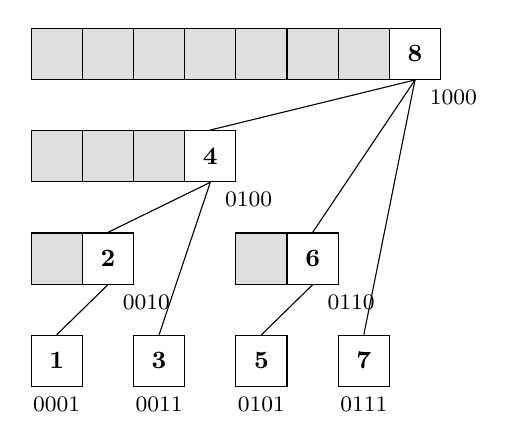
\begin{tikzpicture}[
				x=0.65cm, y=0.65cm,
				cell/.style={draw, minimum width=0.65cm, minimum height=0.65cm,
				inner sep=0pt, font=\small\bfseries},
				gcell/.style={cell, fill=gray!25},
				icell/.style={cell, fill=white},
				binl/.style={font=\footnotesize, inner sep=2pt}
			]
				% 各层 y 坐标
				\def\ya{0}
				\def\yb{2}
				\def\yc{4}
				\def\yd{6}

				% 底层（i 为奇数，lowbit = 1）
				\node[icell] (n1) at (1,\ya) {1};
				\node[icell] (n3) at (3,\ya) {3};
				\node[icell] (n5) at (5,\ya) {5};
				\node[icell] (n7) at (7,\ya) {7};
				\node[binl] at (1,\ya-0.85) {0001};
				\node[binl] at (3,\ya-0.85) {0011};
				\node[binl] at (5,\ya-0.85) {0101};
				\node[binl] at (7,\ya-0.85) {0111};

				% 第二层（lowbit = 2）
				\node[gcell]      at (1,\yb) {};
				\node[icell] (n2) at (2,\yb) {2};
				\node[gcell]      at (5,\yb) {};
				\node[icell] (n6) at (6,\yb) {6};
				\node[binl] at (2.75,\yb-0.85) {0010};
				\node[binl] at (6.75,\yb-0.85) {0110};

				% 第三层（lowbit = 4）
				\foreach \x in {1,2,3} \node[gcell] at (\x,\yc) {};
				\node[icell] (n4) at (4,\yc) {4};
				\node[binl] at (4.75,\yc-0.85) {0100};

				% 第四层（lowbit = 8）
				\foreach \x in {1,...,7} \node[gcell] at (\x,\yd) {};
				\node[icell] (n8) at (8,\yd) {8};
				\node[binl] at (8.75,\yd-0.85) {1000};

				% 管辖/合并关系
				\draw (n8.south) -- (n4.north);
				\draw (n8.south) -- (n6.north);
				\draw (n8.south) -- (n7.north);
				\draw (n4.south) -- (n2.north);
				\draw (n4.south) -- (n3.north);
				\draw (n2.south) -- (n1.north);
				\draw (n6.south) -- (n5.north);
			\end{tikzpicture}
		\end{center}

		例如 $\verb|tr[8]|$ 覆盖区间 $[1,8]$，它正好由 $\verb|tr[4]|$（管 $[1,4]$）、$\verb|tr[6]|$（管 $[5,6]$）、$\verb|tr[7]|$（管 $\{7\}$）和 $a_8$ 本身拼成；而 $\verb|tr[4]|$ 又由 $\verb|tr[2]|$、$\verb|tr[3]|$ 和 $a_4$ 拼成。所有 BIT 操作（\verb|add| 沿 \verb|i += lowbit(i)| 向上、\verb|query| 沿 \verb|i -= lowbit(i)| 向左跳）都能从这张图里直接读出来。

		\subsubsection{单点加，区间求和}

		最基础的 BIT：\verb|add(p, x)| 给位置 $p$ 加上 $x$，\verb|query(l, r)| 返回 \verb|a[l]+a[l+1]+...+a[r]|。下面这份在常规功能之外还带两个小工具，前提是数组里只存 $0/1$（常用于维护一个动态可重集的占位表）：

		\begin{itemize}
			\item \verb|findkth(k)|：从左往右数第 $k$ 个 $1$ 所在的位置。
			\item \verb|kthspace(k)|：从左往右数第 $k$ 个 $0$ 所在的位置。
		\end{itemize}

		两者思路一样：在 BIT 上按位倍增地往右走，每到一步判断「这个块里 $1$（或 $0$）的总数够不够吃掉剩下的 $k$」，够就跨过，不够就留在当前位置继续往下走。整个过程 $O(\log n)$。

		\begin{minted}{cpp}
// by znzryb
// 普通的单点修改区间查询树状数组，
// 含有查找第K个空位，第K个元素的功能
// https://www.codechef.com/viewsolution/1179893708
//   查找第K个元素测试
// 第K个空位的测试应该是一道abc的题目，但是当时没保存
struct BIT {
	vector<ll> tr;
	int n;

	inline int lowbit(int x) {
		return x & (-x);
	}

	BIT(int ln) {
		n = ln;
		tr.resize(n + 5, 0);
	}
	BIT() {}

	inline void add(int p, ll x) {
		if (p == 0) return;
		while (p <= n) {
			tr[p] += x;
			p += lowbit(p);
		}
	}

	inline ll query(int l, int r) {
		ll lres = 0, rres = 0;
		l -= 1;
		while (l > 0) {
			lres += tr[l];
			l -= lowbit(l);
		}
		while (r > 0) {
			rres += tr[r];
			r -= lowbit(r);
		}
		return rres - lres;
	}

	// 找到第 k 个元素，要求只能出现 0 和 1
	inline int findkth(int k) {
		int x = 0, sum = 0;
		for (int i = __lg(n); ~i; --i) {
			x += 1 << i;
			if (x >= n || sum + tr[x] >= k) {
				x -= 1 << i;
			} else {
				sum += tr[x];
			}
		}
		// 始终让 cx < k，+1 就是新元素出现的位置
		return x + 1;
	}

	// 找到第 k 个空位，要求只能出现 0 和 1
	inline int kthspace(int k) {
		int cx = 0;
		// 不断缩小步长的搜索
		for (int i = 1 << 20; i > 0; i >>= 1) {
			if (cx + i <= n &&
				lowbit(cx + i) - tr[cx + i] < k) {
				// lowbit(cx+i) - tr[cx+i]
				//   即该 BIT 块内的空位数
				k -= lowbit(cx + i) - tr[cx + i];
				cx += i;
			}
		}
		return cx + 1;
	}
};
		\end{minted}

		\subsubsection{区间加，单点查询}

		BIT 不再维护原数组 \verb|a|，而是维护差分数组 \verb|d[i] = a[i] - a[i-1]|。这样：

		\begin{itemize}
			\item \textbf{区间加} \verb|a[l..r] += x|：只改差分的两个位置，\verb|d[l] += x; d[r+1] -= x;|
			\item \textbf{单点查} \verb|a[p]|：就是差分的前缀和 \verb|d[1] + d[2] + ... + d[p]|，BIT 天然支持。
		\end{itemize}

		所以这一版的 \verb|add(l, r, x)| 就是对差分做两次单点加，\verb|query(p)| 就是差分的前缀和查询。

		\begin{minted}{cpp}
struct BIT {
	// 支持区间修改，单点查询（使用差分实现）
	// https://www.luogu.com.cn/record/221012815
	vector<ll> tr;
	int n;

	ll lowbit(ll x) {
		return x & (-x);
	}

	BIT(int n_) {
		n = n_;
		tr.resize(n, 0);
	}

	// 差分的单点加，内部用
	void add(ll p, ll x) {
		while (p <= n) {
			tr[p] += x;
			p += lowbit(p);
		}
	}

	// 区间加：a[l..r] += x
	//   等价于 d[l] += x, d[r+1] -= x
	void add(ll l, ll r, ll x) {
		r += 1;
		add(l, x);
		add(r, -x);
	}

	// 单点查 a[p] = d[1] + d[2] + ... + d[p]
	ll query(ll p) {
		ll ret = 0;
		while (p) {
			ret += tr[p];
			p -= lowbit(p);
		}
		return ret;
	}
};
		\end{minted}

		\subsubsection{区间加，区间求和}

		继续沿用差分 \verb|d[i] = a[i] - a[i-1]|。区间加依然是两次 \verb|d[l] += x; d[r+1] -= x|。难点在区间和查询，先看怎么算前缀和 \verb|a[1] + a[2] + ... + a[P]|，把每一项用差分展开：

		\begin{minted}{text}
a[1..P] = d[1]
        + d[1] + d[2]
        + d[1] + d[2] + d[3]
        + ...
        + d[1] + d[2] + ... + d[P]

数一下每个 d[i] 出现了几次：
  d[1] 出现 P 次
  d[2] 出现 P-1 次
  ...
  d[i] 出现 (P - i + 1) 次

所以合并起来：
a[1..P] = sum{ d[i] * (P - i + 1), i = 1..P }
        = (P+1) * sum(d[1..P])
            - sum(i * d[i], i = 1..P)
		\end{minted}

		右边两项都是普通的前缀和，各用一个 BIT 就行：\verb|tr1| 存 \verb|d[i]|，\verb|tr2| 存 \verb|i * d[i]|。于是 \verb|query(P) = (P+1) * sum(tr1, P) - sum(tr2, P)|，区间和就是 \verb|query(r) - query(l-1)|。

		区间加 \verb|[l, r] += x| 时，两个 BIT 要同步改：

		\begin{minted}{text}
对 tr1 （存 d[i]）：
  tr1 在 l   处 += x
  tr1 在 r+1 处 -= x

对 tr2 （存 i * d[i]）：
  i = l   时：d[l]   += x  =>  i*d[i] +=   l  * x
  i = r+1 时：d[r+1] -= x  =>  i*d[i] -= (r+1) * x
		\end{minted}

		注意乘的系数 \verb|l|、\verb|r+1| 在修改时就是已知常数，所以能直接塞进 \verb|tr2| 的单点加里。

		\begin{minted}{cpp}

/* 2026-04-19 luogu 线段树模板题
 * AC https://www.luogu.com.cn/record/274702532
 * 进一步添加了 public,private 规定了接口的可见性
 * 2026-04-19 增强了对 0 的鲁棒性
 * AC https://acm.hdu.edu.cn/contest/view-code?cid=1201&rid=9803
 */
 class BIT {
	// 支持区间修改，区间查询
	// 维护两个差分：d[i] 和 i*d[i]
	// 前缀和 sum(p) = (p+1)*sum(d[1..p])
	//              - sum(i*d[i], 1..p)
	vector<ll> tr1, tr2;
	int n;

	ll lowbit(ll x) {
		return x & (-x);
	}

public:
	BIT(int n_) {
		n = n_;
		// 这个 n+1 就够了，虽然涉及到这个差分
		tr1.assign(n + 2, 0);
		tr2.assign(n + 2, 0);
	}

private:
	void add(vector<ll> &tr, ll p, ll x) {
		// 防止 0 死循环
		if (p <= 0) return;
		while (p <= n) {
			tr[p] += x;
			p += lowbit(p);
		}
	}

	ll sum(vector<ll> &tr, ll p) {
		ll ret = 0;
		while (p) {
			ret += tr[p];
			p -= lowbit(p);
		}
		return ret;
	}

	// 单点加
	void add(ll p, ll x) {
		add(tr1, p, x);
		add(tr2, p, p * x);
	}

public:
	// 区间加，[l, r] 每个位置加 x
	void add(ll l, ll r, ll x) {
		add(tr1, l, x);
		add(tr1, r + 1, -x);
		add(tr2, l, l * x);
		add(tr2, r + 1, -(r + 1) * x);
	}

private:
	// 前缀和 a[1] + a[2] + ... + a[p]
	ll query(ll p) {
		return (p + 1) * sum(tr1, p) - sum(tr2, p);
	}

public:
	// 区间和 a[l] + ... + a[r]
	ll query(ll l, ll r) {
		return query(r) - query(l - 1);
	}
};
		\end{minted}

		\paragraph{技巧：提前结算避免树状数组清零}

		\href{https://acm.hdu.edu.cn/contest/problem?cid=1201&pid=1007}{从这道题目学到的技巧}

		树状数组不支持高效的区间清零（需要逐点撤销）。但如果我们知道某段区间 $[l, r]$ 上累积的值最终要\textbf{贡献给谁}，就可以在需要“清零”的时刻，先把 BIT 上 $[l, r]$ 的当前和查出来、结算到对应的答案里，然后\textbf{不做任何清零操作}。之后 BIT 上再产生的增量会叠加在旧值之上，但因为旧值已经被结算走了，所以只要在最终统计时再查一次并减去"已结算部分"，效果就等价于清零后重新累加。

		典型场景：维护若干组的区间贡献，当某段区间的归属从旧组切换到新组时：

		\begin{minted}{cpp}
// 将 [l, r] 的归属从 originV 切换到 val，不清零 BIT
ll add = tr->query(l, r);   // 查出 [l, r] 上的已有增量
anss[originV] += add;        // 旧归属结算
anss[val] -= add;            // 新归属预扣（之后查询时会连带查出这部分旧值）
		\end{minted}

		\subsubsection{单点改，区间最值查询（BIT 实现 RMQ）}

		和求和不同，$\min / \max$ 这类运算\textbf{只有结合律、没有逆运算}（即没有「区间减法」），所以不能像前缀和那样用 $\text{pre}(r) - \text{pre}(l-1)$ 直接拿到任意区间的结果。不过 BIT 的分块结构只依赖结合律就够用了：每个 \verb|tr[i]| 管辖 \verb|a[i - lowbit(i) + 1 .. i]| 这个区间的最值，因此整个骨架仍然可以复用，只是查询和更新都必须按块拼凑，复杂度从 $O(\log n)$ 退化到 $O(\log^2 n)$。相对于 ST 表的优势是\textbf{支持在线单点修改}。

		\textbf{查询} \verb|query(l, r)|：从右端 \verb|r| 往左跳，每次能吃掉一整个 BIT 块就吃（\verb|tr[r]|，跨度 \verb|lowbit(r)|），吃不动的那一格（即 \verb|r - lowbit(r) < l| 的时候）退化为单独看 \verb|a[r]|，然后 \verb|r--| 继续：

		\begin{minted}{text}
res = dummy
while r >= l:
    res = op(res, a[r])        // 单独处理 a[r]
    r -= 1
    while r - lowbit(r) >= l:   // 尽量用 BIT 块跳
        res = op(res, tr[r])
        r -= lowbit(r)
		\end{minted}

		\textbf{更新} \verb|upd(p, x)|：把 \verb|a[p]| 覆盖为 \verb|x| 之后，所有「管辖 \verb|p| 的 BIT 块」都要重算。这些块的下标就是

		\begin{minted}{text}
i = p,
    p + lowbit(p),
    p + lowbit(p) + lowbit(p + lowbit(p)),
    ...
		\end{minted}

		也就是外层循环 \verb|i += lowbit(i)| 依次枚举的那些位置。由于没有区间减法，无法从旧 \verb|tr[i]| 里扣掉旧 \verb|a[p]| 的贡献，所以只能\textbf{从头合并整块}。

		好在 BIT 的管辖区间有一个漂亮的自相似分解——它能切成若干长度是 $2$ 的幂、两两不相交的子段，而这些子段本身就是已有的更小的 \verb|tr|：

		\begin{minted}{text}
tr[i] 管辖 [i - lowbit(i) + 1 .. i]，长度 lowbit(i)
可拆成：
    tr[i - lowbit(i)/2]    长度 lowbit(i)/2   // 左半
    tr[i - lowbit(i)/4]    长度 lowbit(i)/4   // 再右半的一半
    ...
    tr[i - 2]              长度 2
    tr[i - 1]              长度 1
    a[i]                   长度 1             // 自己这一格

验证：1 + 1 + 2 + 4 + ... + lowbit(i)/2 = lowbit(i)
      刚好铺满管辖区间。
		\end{minted}

		所以重算就是：

		\begin{minted}{text}
tr[i] = op(a[i],
           tr[i - 1],
           tr[i - 2],
           tr[i - 4],
           ...,
           tr[i - lowbit(i)/2])
		\end{minted}

		对应代码里的内层循环——让 \verb|j| 从 $1$ 按 $2$ 的幂翻倍直到 \verb|lowbit(i)/2|。

% \textbf{为什么 \texttt{tr[i - j]} 直接用旧值就对？}  把所有用到的小块按「管辖区间是否含 \verb|p|」分成两类：
% \begin{itemize}
% 	\item 含 \verb|p| 的：它一定是本轮外层循环在更早的某次迭代里刚被重算过的——因为 \verb|i += lowbit(i)| 保证我们总是\textbf{先处理更小的 i}，而含 \verb|p| 的那个小块的下标一定小于当前 \verb|i|。
% 	\item 不含 \verb|p| 的：它的值自始至终没变，自然是最新的。
% \end{itemize}

% 两种情况下 \verb|tr[i - j]| 都已经是最新值。单次 \verb|upd| 的复杂度：外层 $O(\log n)$ 次、每次内层合并至多 $O(\log n)$ 个小块，总共 $O(\log^2 n)$。

		\begin{minted}{cpp}
// by Gospel_rock znzryb
// 参考了（抄了）OIwiki
// AC https://www.luogu.com.cn/record/228807838
//   （ST 表模版题，max 版本）
// AC https://www.luogu.com.cn/record/228809172
//   （打乱了插入顺序，同题）
// AC https://codeforces.com/contest/2184/submission/358028437
// 进行了现代化改造，更加符合现在我们的习惯
struct RMQ {
	const ll dummy = INF;
	ll n;
	vector<ll> tr;
	vector<ll> origin;

	inline ll lowbit(const ll &x) {
		return x & -x;
	}

private:
	ll op(const ll &a, const ll &b) {
		return min(a, b);
	}

public:
	RMQ(ll n) {
		this->n = n + 2;
		tr.resize(n + 5, INF);
		origin.resize(n + 5);
	}

	ll query(ll l, ll r) {
		ll res = dummy;
		while (r >= l) {
			res = op(origin[r], res);
			r--;
			for (; r - lowbit(r) >= l; r -= lowbit(r)) {
				res = op(res, tr[r]);
			}
		}
		return res;
	}

	// 注意：语义是「把位置 p 覆盖为 x」，不是增加
	void upd(ll p, ll x) {
		origin[p] = x;
		for (int i = p; i <= n; i += lowbit(i)) {
			tr[i] = origin[i];
			for (int j = 1; j < lowbit(i); j <<= 1) {
				tr[i] = op(tr[i], tr[i - j]);
			}
		}
	}
};
		\end{minted}

		\textbf{切换 \texttt{min}/\texttt{max}}：把 \verb|op| 改成 \verb|max|、同时把 \verb|dummy| 从 \verb|INF| 改成 \verb|-INF| 即可。如果要泛化成任意幂等运算（操作一次和操作十次结果一样如，\verb|gcd|、按位与/或等），需要选一个对该运算「吸收」的恒元作为 \verb|dummy|。

		\subsection{珂朵莉树（ODT / Chtholly Tree）}

		珂朵莉树用 \verb|std::map| 维护若干不相交的「颜色段」\verb|[l, r, val]|。核心思路：\textbf{每次区间赋值把覆盖到的所有旧段一次性合并删除}，再插入一段新段。在随机数据或有大量区间覆盖操作的题目中，段数期望 $O(n \log n)$，因此总复杂度可接受。

		两个核心操作：
		\begin{itemize}
			\item \verb|split(pos)|：把包含 \verb|pos| 的段在 \verb|pos| 处切开，保证 \verb|pos| 是某段的左端点。
			\item \verb|assign(la, ra, val)|：先 \verb|split| 两端，然后一次性抹掉 $[la, ra]$ 内所有旧段，插入新段。在抹掉每段时可顺带做任意聚合统计（如下方用 BIT 查区间权重和并累到 \verb|anss| 上）。
		\end{itemize}

		\begin{minted}{cpp}
	/*
	 * 2026-04-19 内部式的 ODT
	 * AC https://acm.hdu.edu.cn/contest/view-code?cid=1201&rid=9850
	 */
	struct RVal {
		ll r;
		ll val;
	};

	map<ll, RVal> mpODT;

	void split(ll pos) {
		if (mpODT.empty()) return;
		auto it = mpODT.upper_bound(pos);
		if (it == mpODT.begin()) return;
		it--;
		// pos 就是左端点         pos 不在区间内
		if (it->first == pos || it->second.r < pos) {
			return;
		}
		mpODT[pos] = {it->second.r, it->second.val};
		it->second.r = pos - 1;
	}

	void assign(ll la, ll ra, ll val) {
		split(la);
		split(ra + 1);
		auto it = mpODT.lower_bound(la);
#ifdef LOCAL
		assert(it->first==la);
#endif
		for (; it != mpODT.end();) {
			if (it->first > ra) {
				break;
			}
			ll originV = it->second.val;
			ll l = it->first, r = it->second.r;
			// 这里是做一些事情，比如说累加答案
			// ll add = tr->query(l, r);
			// anss[originV] += add;
			// anss[val] -= add;
			it = mpODT.erase(it);
		}
		mpODT[la] = {ra, val};
	}
		\end{minted}

		\subsection{懒标记线段树（Tag + Info 写法）}

		加和线段树常见写法（队友的模版）。把节点信息抽成 \verb|Info|、懒标记抽成 \verb|Tag|，线段树本体只负责 \verb|pushUp| / \verb|pushDown| / \verb|apply| 的递归骨架，具体语义全部由 \verb|Info::apply(tag, l, r)|、\verb|Tag::apply(tag)|、\verb|Tag::empty()|、\verb|Info::operator+| 这几个接口提供。换不同的 \verb|Info| / \verb|Tag| 就能复用同一棵树。

		\begin{minted}{cpp}
template <class InfoType = Info, class TagType = Tag>
class LazySegmentTree
{
  int n;
  vector<InfoType> tree;
  vector<TagType> lazy;

  void pushUp(int id)
  {
    tree[id] = tree[id << 1] + tree[id << 1 | 1];
  }

  void apply(int id, int l, int r, const TagType &tag)
  {
    tree[id].apply(tag, l, r);
    lazy[id].apply(tag);
  }

  void pushDown(int id, int l, int r)
  {
    if (lazy[id].empty())
    {
      return;
    }

    int mid = (l + r) >> 1;
    apply(id << 1, l, mid, lazy[id]);
    apply(id << 1 | 1, mid + 1, r, lazy[id]);
    lazy[id] = TagType();
  }

  void build(int id, int l, int r, const vector<InfoType> &a)
  {
    if (l == r)
    {
      tree[id] = a[l];
      return;
    }

    int mid = (l + r) >> 1;
    build(id << 1, l, mid, a);
    build(id << 1 | 1, mid + 1, r, a);
    pushUp(id);
  }

  void modify(int id, int l, int r, int ql, int qr, const TagType &tag)
  {
    if (ql <= l && r <= qr)
    {
      apply(id, l, r, tag);
      return;
    }

    pushDown(id, l, r);

    int mid = (l + r) >> 1;

    if (ql <= mid)
    {
      modify(id << 1, l, mid, ql, qr, tag);
    }

    if (qr > mid)
    {
      modify(id << 1 | 1, mid + 1, r, ql, qr, tag);
    }

    pushUp(id);
  }

  InfoType query(int id, int l, int r, int ql, int qr)
  {
    if (ql <= l && r <= qr)
    {
      return tree[id];
    }

    pushDown(id, l, r);

    int mid = (l + r) >> 1;

    if (qr <= mid)
    {
      return query(id << 1, l, mid, ql, qr);
    }

    if (ql > mid)
    {
      return query(id << 1 | 1, mid + 1, r, ql, qr);
    }

    return query(id << 1, l, mid, ql, qr) +
           query(id << 1 | 1, mid + 1, r, ql, qr);
  }

public:
  LazySegmentTree(int n = 0)
  {
    init(n);
  }

  LazySegmentTree(const vector<InfoType> &a)
  {
    build(a);
  }

  void init(int n_)
  {
    n = n_;
    tree.assign(4 * n + 5, InfoType());
    lazy.assign(4 * n + 5, TagType());
  }

  void build(const vector<InfoType> &a)
  {
    init((int)a.size() - 1);

    if (n > 0)
    {
      build(1, 1, n, a);
    }
  }

  void modify(int l, int r, const TagType &tag)
  {
    if (l > r)
    {
      return;
    }

    modify(1, 1, n, l, r, tag);
  }

  InfoType query(int l, int r)
  {
    return query(1, 1, n, l, r);
  }
};
		\end{minted}

		\subsection{带权可撤销并查集（判二分图）}

		带权可撤销并查集（队友的模版），可以用来判断图是否是二分图。\textbf{一般和线段树分治绑定}：分治进入子区间前 \verb|snapshot()|，离开时 \verb|rollback()| 回到该快照，省去为每个时间区间重建图的代价。\verb|val[x]| 维护 \verb|x| 到 \verb|fa[x]| 的边权异或值，\verb|find| 不做路径压缩（路径压缩与回滚不兼容），靠按秩合并保 $O(\log n)$ 单次。\verb|badCnt| 计数当前累计的「奇环」（合并时 \verb|valx ^ valy != w| 即一条奇环），\verb|isBipartiteGraph()| 即 \verb|badCnt == 0|。

		\begin{minted}{cpp}
class RollbackDSU
{
  struct Info
  {
    int x, y, oldSizeY, oldBadCnt, oldValX;
    bool isMerged;
  };

  int badCnt;
  vector<int> fa, sz, val;
  stack<Info> history;

public:
  RollbackDSU(int n) : badCnt(0), fa(n + 1), sz(n + 1, 1), val(n + 1, 0)
  {
    iota(fa.begin(), fa.end(), 0);
  }

  int snapshot()
  {
    return (int)history.size();
  }

  void rollback(int snapshot)
  {
    while ((int)history.size() > snapshot)
    {
      auto [x, y, oldSizeY, oldBadCnt, oldValX, isMerged] = history.top();
      history.pop();

      badCnt = oldBadCnt;

      if (!isMerged)
      {
        continue;
      }

      val[x] = oldValX;
      sz[y] = oldSizeY;
      fa[x] = x;
    }
  }

  pair<int, int> find(int x)
  {
    int cur = 0;

    while (fa[x] != x)
    {
      cur ^= val[x];
      x = fa[x];
    }

    return {x, cur};
  }

  bool merge(int x, int y, int w)
  {
    auto [fx, valx] = find(x);
    auto [fy, valy] = find(y);

    if (fx == fy)
    {
      history.push({0, 0, 0, badCnt, 0, false});

      if ((valx ^ valy) != w)
      {
        badCnt++;
      }

      return false;
    }

    if (sz[fx] > sz[fy])
    {
      swap(fx, fy);
      swap(valx, valy);
    }

    history.push({fx, fy, sz[fy], badCnt, val[fx], true});

    sz[fy] += sz[fx];
    val[fx] = valx ^ valy ^ w;
    fa[fx] = fy;

    return true;
  }

  bool isBipartiteGraph() const
  {
    return badCnt == 0;
  }
};
		\end{minted}

		\subsection{线段树分治}

		线段树分治模板（队友的模版），常和上面的可撤销带权并查集绑定，用来\textbf{离线处理「在时间轴上每条边只在区间 $[l, r]$ 内存在」类型的问题}。把每条边按其存活时间区间挂到线段树对应的若干 $O(\log q)$ 个节点上；DFS 整棵线段树，进入节点前依次 \verb|merge| 该节点上挂的所有边，离开节点前 \verb|rollback| 到进入时的 \verb|snapshot|，到叶子时即可拿到该时间点的并查集状态（如查二分图：\verb|isBipartiteGraph()|）。

		\begin{minted}{cpp}
struct SegmentTreeDivide {
  int q;
  vector<vector<pair<int, int>>> seg;

  SegmentTreeDivide() {}

  SegmentTreeDivide(int q) {
    init(q);
  }

  void init(int q_) {
    q = q_;
    seg.assign(4 * q + 5, {});
  }

  void add(int node, int l, int r, int ql, int qr, pair<int, int> edge) {
    if (ql <= l && r <= qr) {
      seg[node].push_back(edge);
      return;
    }

    int mid = (l + r) >> 1;

    if (ql <= mid) {
      add(node << 1, l, mid, ql, qr, edge);
    }

    if (qr > mid) {
      add(node << 1 | 1, mid + 1, r, ql, qr, edge);
    }
  }

  void add(int l, int r, pair<int, int> edge) {
    if (l > r) {
      return;
    }

    add(1, 1, q, l, r, edge);
  }
};
		\end{minted}

		\subsection{zkw线段树}

		\subsubsection{zkw线段树区间加}
		\begin{minted}{cpp}
// 参考zkw的PPT 以及 https://www.luogu.com.cn/record/207546670
// 参考题解 https://www.luogu.com.cn/article/w3gfeebh
// AC https://www.luogu.com.cn/record/232855513 区间加
constexpr ll preset=0;
struct SEG{
    static ll op(const ll &a,const ll &b){
        return a+b;
    }
    int n,sz=1,dep;
    vector<ll> tr;vector<ll> tag;
    SEG(int n){     // 传入的时候可以传大一点
        this->n=n+2;
        dep=__lg(this->n)+1;
        sz=1<<dep;
        tr.resize((sz<<1)+5,preset);
        tag.resize((sz<<1)+5,preset);
    }
    int len(int o){return 1<<(dep-__lg(o));}
    void pushup(int o){tr[o]=op(tr[o<<1],tr[o<<1|1]);}
    void settag(int o,ll x){
        tr[o]=op(tr[o],len(o)*x);
        tag[o]=op(tag[o],x);
    }
    void pushdown(int o){
        int l=o<<1,r=l|1;   // 左儿子，右儿子
        settag(l, tag[o]);
        settag(r, tag[o]);
        tag[o]=0;
    }
    void assign(int i,ll x){
        tr[i+sz]=x;
    }
    void build(){
        for(int o=sz-1;o>=1;--o){
            pushup(o);
        }
    }
    void push(int l,int r){
        //        在j层，l，r变为了同一点
        int i=dep,j=__lg(l^r);
        while (i>j) {   // 就是为了避免一下重复下推
            pushdown(l>>i--);
        }
        while(i){
            pushdown(l>>i),pushdown(r>>i--);
        }
    }
    ll query(int l,int r){
        ll res=preset;
        // 变为开区间，并加上sz
        l=l-1+sz,r=r+1+sz;
        push(l,r);
        for(;l^r^1;l>>=1,r>>=1){
            // l^r^1 表示 只要 l 与 r 还不是同一个父亲的两兄弟，就继续上跳。
            if(~l&1){   
                // l是偶数，说明l是父节点的左儿子，开区间，将其右儿子加入答案
                res=op(res,tr[l^1]);
            }
            if(r&1){
                res=op(tr[r^1],res);
            }
        }
        return res;
    }
    void add(int l,int r,ll x){
        l=l-1+sz,r=r+1+sz;
        push(l, r);
        for(;l^r^1;pushup(l>>=1),pushup(r>>=1)){
            if(~l&1){
                settag(l^1, x);
            }
            if(r&1){
                settag(r^1, x);
            }
        }
        for (l >>= 1; l; l >>= 1) pushup(l);
    }
};
		\end{minted}

		\subsubsection{线段树区间加乘（递归 / zkw）}
		\href{https://www.luogu.com.cn/record/177481404}{www.luogu.com.cn}
		\begin{minted}{cpp}
// 参考zkw的PPT 以及 https://www.luogu.com.cn/record/207546670
// 参考题解 https://www.luogu.com.cn/article/w3gfeebh
// AC https://www.luogu.com.cn/record/232855282 线段树区间加乘
constexpr ll preset=0;
// 依赖常量mod
struct SEG{
    int n,sz=1,dep;
    static ll op(const ll &a,const ll &b){
        return (a+b)%mod;
    }
    vector<ll> tr;vector<ll> tag;vector<ll> tag2;
    SEG(int n){     // 传入的时候可以传大一点
        this->n=n+2;
        dep=__lg(this->n)+1;
        sz=1<<dep;
        tr.resize((sz<<1)+5,preset);
        tag.resize((sz<<1)+5,preset);
        tag2.resize((sz<<1)+5,1);
    }
    int len(int o){return 1<<(dep-__lg(o));};
    void pushup(int o){tr[o]=op(tr[o<<1],tr[o<<1|1]);}
    void settag(int o,ll x){
        tr[o]=op(tr[o],x*len(o));
        tag[o]=op(tag[o],x);
    }
    void settag2(int o,ll x){
        tr[o]=op(tr[o]*x,0);
        tag[o]=op(tag[o]*x,0);
        tag2[o]=op(tag2[o]*x,0);
    }
    void pushdown(int o){
        int l=o<<1,r=l|1;   // 左儿子，右儿子
        if(tag2[o]!=1){
            settag2(l, tag2[o]);
            settag2(r, tag2[o]);
            tag2[o]=1;
        }
        if(tag[o]!=0){
            settag(l, tag[o]);
            settag(r, tag[o]);
            tag[o]=0;
        }
    }
    void assign(int i,ll x){
        tr[i+sz]=x;
    }
    void build(){
        for(int o=sz-1;o>=1;--o){
            pushup(o);
        }
    }
    void push(int l,int r){
        //        在j层，l，r变为了同一点
        int i=dep,j=__lg(l^r);
        while (i>j) {   // 就是为了避免一下重复下推
            pushdown(l>>i--);
        }
        while(i){
            pushdown(l>>i),pushdown(r>>i--);
        }
    }
    ll query(int l,int r){
        ll res=preset;
        // 变为开区间，并加上sz
        l=l-1+sz,r=r+1+sz;
        push(l,r);
        for(;l^r^1;l>>=1,r>>=1){
            // l^r^1 表示 只要 l 与 r 还不是同一个父亲的两兄弟，就继续上跳。
            if(~l&1){   
                // l是偶数，说明l是父节点的左儿子，开区间，将其右儿子加入答案
                res=op(res,tr[l^1]);
            }
            if(r&1){
                res=op(tr[r^1],res);
            }
        }
        return res;
    }
    void add(int l,int r,ll x){
        l=l-1+sz,r=r+1+sz;
        push(l, r);
        for(;l^r^1;pushup(l>>=1),pushup(r>>=1)){
            if(~l&1){
                settag(l^1, x);
            }
            if(r&1){
                settag(r^1, x);
            }
        }
        for (l >>= 1; l; l >>= 1) pushup(l);
    }
    void mul(int l,int r,ll x){
        l=l-1+sz,r=r+1+sz;
        push(l, r);
        for(;l^r^1;pushup(l>>=1),pushup(r>>=1)){
            if(~l&1){
                settag2(l^1, x);
            }
            if(r&1){
                settag2(r^1, x);
            }
        }
        for (l >>= 1; l; l >>= 1) pushup(l);
    }
};
		\end{minted}

		\subsubsection{zkw区间推平+-，区间和查询}
		\begin{minted}{cpp}
// 参考zkw的PPT 以及 https://www.luogu.com.cn/record/207546670
// 参考题解 https://www.luogu.com.cn/article/w3gfeebh
// AC https://atcoder.jp/contests/abc417/submissions/68719700 线段树区间加减，区间修改，区间和查询
constexpr ll preset=0,initv=-INF;
// 依赖常量mod   线段树区间加减，区间修改，区间和查询
struct SEG{
    int n,sz=1,dep;
    static ll op(const ll &a,const ll &b){
        return (a+b)%mod;
    }
    vector<ll> tr;vector<ll> tag;vector<ll> tag2;
    SEG(int n){     // 传入的时候可以传大一点
        this->n=n+2;
        dep=__lg(this->n)+1;
        sz=1<<dep;
        tr.resize((sz<<1)+5,preset);
        tag.resize((sz<<1)+5,preset);
        tag2.resize((sz<<1)+5,initv);
    }
    int len(int o){return 1<<(dep-__lg(o));};
    void pushup(int o){tr[o]=op(tr[o<<1],tr[o<<1|1]);}
    void settag(int o,ll x){
        tr[o]=op(tr[o],x*len(o));
        tag[o]=op(tag[o],x);
    }
    void settag2(int o,ll x){
        tr[o]=op(len(o)*x,0);
        tag[o]=0;
        tag2[o]=x;
    }
    void pushdown(int o){
        int l=o<<1,r=l|1;   // 左儿子，右儿子
        if(tag2[o]!=initv){
            settag2(l, tag2[o]);
            settag2(r, tag2[o]);
            tag2[o]=initv;
        }
        if(tag[o]!=0){
            settag(l, tag[o]);
            settag(r, tag[o]);
            tag[o]=0;
        }
    }
    void assign(int i,ll x){
        tr[i+sz]=x;
    }
    void build(){
        for(int o=sz-1;o>=1;--o){
            pushup(o);
        }
    }
    void push(int l,int r){
        //        在j层，l，r变为了同一点
        int i=dep,j=__lg(l^r);
        while (i>j) {   // 就是为了避免一下重复下推
            pushdown(l>>i--);
        }
        while(i){
            pushdown(l>>i),pushdown(r>>i--);
        }
    }
    ll query(int l,int r){
        ll res=preset;
        // 变为开区间，并加上sz
        l=l-1+sz,r=r+1+sz;
        push(l,r);
        for(;l^r^1;l>>=1,r>>=1){
            // l^r^1 表示 只要 l 与 r 还不是同一个父亲的两兄弟，就继续上跳。
            if(~l&1){   
                // l是偶数，说明l是父节点的左儿子，开区间，将其右儿子加入答案
                res=op(res,tr[l^1]);
            }
            if(r&1){
                res=op(tr[r^1],res);
            }
        }
        return res;
    }
    void add(int l,int r,ll x){
        l=l-1+sz,r=r+1+sz;
        push(l, r);
        for(;l^r^1;pushup(l>>=1),pushup(r>>=1)){
            if(~l&1){
                settag(l^1, x);
            }
            if(r&1){
                settag(r^1, x);
            }
        }
        for (l >>= 1; l; l >>= 1) pushup(l);
    }
    void modify(int l,int r,ll x){
        l=l-1+sz,r=r+1+sz;
        push(l, r);
        for(;l^r^1;pushup(l>>=1),pushup(r>>=1)){
            if(~l&1){
                settag2(l^1, x);
            }
            if(r&1){
                settag2(r^1, x);
            }
        }
        for (l >>= 1; l; l >>= 1) pushup(l);
    }
};
		\end{minted}

		\subsubsection{zkwlen}
		\begin{minted}{cpp}
int dis(int o){return dep-__lg(o);}
int len(int o){return 1<<dis(o);}
int le(int o){return (o<<dis(o))-sz;}
int rr(int o){return (o+1<<dis(o))-sz-1;}
		\end{minted}

		\subsubsection{线段树RMQ（zkw / 递归式）}
		\begin{minted}{cpp}
// 参考zkw的PPT 以及 https://www.luogu.com.cn/record/207546670
// 参考题解 https://www.luogu.com.cn/article/w3gfeebh
// AC https://www.luogu.com.cn/record/232824635 RMQ 
// AC https://acm.hdu.edu.cn/contest/view-code?cid=1178&rid=19433 6s 以内
constexpr ll preset=-INF;
struct SEG{
    static ll op(const ll &a,const ll &b){
        return max(a,b);
    }
    int n,sz=1,dep;
    vector<ll> tr;vector<ll> tag;vector<bool> fixed;
    SEG(int n){     // 传入的时候可以传大一点
        this->n=n+2;
        dep=__lg(this->n)+1;
        sz=1<<dep;
        tr.resize((sz<<1)+5,preset);
        tag.resize((sz<<1)+5,0);
        fixed.resize((sz<<1)+5,false);
    }
    void pushup(int o){tr[o]=op(tr[o<<1],tr[o<<1|1]);}
    void settag(int o,ll x){
        tr[o]+=x;
        if(!fixed[o]) tag[o]+=x;
    }
    void settag2(int o,ll x){   // 覆盖
        tr[o]=x;
        tag[o]=0;
        fixed[o]=true;
    }
    void pushdown(int o){ 
        int l=o<<1,r=l|1;   // 左儿子，右儿子
        if(fixed[o]){
            settag2(l, tr[o]);
            settag2(r, tr[o]);
            fixed[o]=false;
        }
        if(tag[o]){
            settag(l, tag[o]);
            settag(r, tag[o]);
            tag[o]=0;
        }
    }
    void push(int l,int r){
        //        在j层，l，r变为了同一点
        int i=dep,j=__lg(l^r);
        while (i>j) {   // 就是为了避免一下重复下推
            pushdown(l>>i--);
        }
        while(i){
            pushdown(l>>i),pushdown(r>>i--);
        }
    }
    void assign(int i,ll x){   
        tr[i+sz]=x;
    }
    void build(){
        for(int o=sz-1;o>=1;--o){
            pushup(o);
        }
    }
    ll query(int l,int r){
        ll res=preset;
        // 变为开区间，并加上sz
        l=l-1+sz,r=r+1+sz;
        push(l,r);
        for(;l^r^1;l>>=1,r>>=1){
            // l^r^1 表示 只要 l 与 r 还不是同一个父亲的两兄弟，就继续上跳。
            if(~l&1){   
                // l是偶数，说明l是父节点的左儿子，开区间，将其右儿子加入答案
                res=op(res,tr[l^1]);
            }
            if(r&1){
                res=op(tr[r^1],res);
            }
        }
        return res;
    }
    void add(int l,int r,ll x){
        int w=1;
        l=l-1+sz,r=r+1+sz;
        push(l, r);
        for(;l^r^1;pushup(l>>=1),pushup(r>>=1),w<<=1){
            if(~l&1){
                settag(l^1, x);
            }
            if(r&1){
                settag(r^1, x);
            }
        }
        for (l >>= 1; l; l >>= 1) pushup(l);
    }
    void modify(int l,int r,ll x){
        int w=1;
        l=l-1+sz,r=r+1+sz;
        push(l, r);
        for(;l^r^1;pushup(l>>=1),pushup(r>>=1),w<<=1){
            if(~l&1){
                settag2(l^1, x);
            }
            if(r&1){
                settag2(r^1, x);
            }
        }
        for (l >>= 1; l; l >>= 1) pushup(l);
    }
};
		\end{minted}

		\subsubsection{zkw 小白逛公园（维护最大子段和）}
		\begin{minted}{cpp}
// 参考了（抄了）beta99999 的提交  https://www.luogu.com.cn/record/216441078
// 因为自己重写的，目前只支持zkw线段树，配置上只保留了identity
// 采用0-based，左开右闭区间，注意这个区间转化
// AC https://www.luogu.com.cn/record/230419677 最大子段和
template <typename T,typename value_type> struct base_segtree{
    int n,sz;
    vector<value_type> tr;
    static int bit_ceil(int x){int res=1;while(res<x){res<<=1;} return res;};
    // zkw线段树开两倍大小，identity为默认值
    base_segtree(int n):n(n),sz(bit_ceil(n)),tr((sz<<1),T::identity){}    
    T *derived() { return static_cast<T*>(this); }
    void pushup(int o){
        tr[o]=T::op(tr[o<<1],tr[o<<1|1]);
    }

    // zkw选配  
    int dis(int o){return __lg(sz)-__lg(o);}    // 倒数第几层？有倒数第0层
    int len(int o){return 1<<dis(o);}   // （直接调用就可以，就是左闭右开区间长度）
    int le(int o){return (o<<dis(o))-sz; }  // 左闭
    int rr(int o){return (o+1<<dis(o))-sz;} // 右开
    void build(){
        for(int o=sz-1;o>=1;--o){
            derived()->pushup(o);
        }
    }
    template<typename D> 
    void update(int l,D x){
        tr[l+sz]=x;
        int o=l+sz;
        for(int i=1;i<=__lg(o);++i){
            derived()->pushup(o>>i);
        }
    }
    value_type query(int l, int r){
        l+=sz;r+=sz;    // T:: 调用的是类的静态成员，无需实例化
        value_type resl=T::identity,resr=T::identity;
        for(;l<r;l>>=1,r>>=1){
            if(l&1) resl=T::op(resl,tr[l++]);
            if(r&1) resr=T::op(tr[--r],resr);
        }
        return T::op(resl,resr);
    }
    void assign(int i,value_type a){
        tr[i+sz]=a;
    }
};
struct State{
    ll pre,suf,mx,sum;
    // State(ll pre,ll suf,ll mx,ll sum):pre(pre),suf(suf),mx(mx),sum(sum) {}
};
struct segtree:base_segtree<segtree, State>{
    static constexpr State identity={-INF,-INF,-INF,0};
    static State op(const State &a,const State &b){
        return {
            max(b.pre+a.sum,a.pre),
            max(b.suf,b.sum+a.suf),
            max({a.mx,b.mx,a.suf+b.pre}),
            a.sum+b.sum
        };
    }
    segtree(ll n):base_segtree<segtree, State>(n){}
};
constexpr State segtree::identity;
		\end{minted}

		\subsubsection{zkw线段树维护平方和}
		\begin{minted}{cpp}
// 参考zkw的PPT 以及 https://www.luogu.com.cn/record/207546670
// 参考题解 https://www.luogu.com.cn/article/w3gfeebh
// AC https://www.luogu.com.cn/record/232879230 线段树区间加减，区间修改，区间和查询
constexpr ll preset=0,initv=-INF;
// 依赖常量mod   线段树区间加减，区间修改，区间和查询
struct SEG{
    int n,sz=1,dep;
    static ll op(const ll &a,const ll &b){
        return (a+b);
    }
    vector<ll> tr;vector<ll> tag;vector<ll> tag2;
    vector<ll> sum;
    SEG(int n){     // 传入的时候可以传大一点
        this->n=n+2;
        dep=__lg(this->n)+1;
        sz=1<<dep;
        tr.resize((sz<<1)+5,preset);
        tag.resize((sz<<1)+5,preset);
        tag2.resize((sz<<1)+5,initv);
        sum.resize((sz<<1)+5,preset);
    }
    int len(int o){return 1<<(dep-__lg(o));};
    void pushup(int o){
        tr[o]=op(tr[o<<1],tr[o<<1|1]);
        sum[o]=op(sum[o<<1],sum[o<<1|1]);
    }
    void settag(int o,ll x){
        tr[o]=op(tr[o],x*x*len(o)+sum[o]*x*2);
        sum[o]=op(sum[o],x*len(o));
        tag[o]=op(tag[o],x);
    }
    void settag2(int o,ll x){
        tr[o]=op(len(o)*x*x,0);
        sum[o]=op(x*len(o),0);
        tag[o]=0;
        tag2[o]=x;
    }
    void pushdown(int o){
        int l=o<<1,r=l|1;   // 左儿子，右儿子
        if(tag2[o]!=initv){ 
            settag2(l, tag2[o]);
            settag2(r, tag2[o]);
            tag2[o]=initv;
        }
        if(tag[o]!=0){
            settag(l, tag[o]);
            settag(r, tag[o]);
            tag[o]=0;
        }
    }
    void assign(int i,ll x){
        tr[i+sz]=x*x;
        sum[i+sz]=x;
    }
    void build(){
        for(int o=sz-1;o>=1;--o){
            pushup(o);
        }
    }
    void push(int l,int r){
        //        在j层，l，r变为了同一点
        int i=dep,j=__lg(l^r);
        while (i>j) {   // 就是为了避免一下重复下推
            pushdown(l>>i--);
        }
        while(i){
            pushdown(l>>i),pushdown(r>>i--);
        }
    }
    ll query(int l,int r){
        ll res=preset;
        // 变为开区间，并加上sz
        l=l-1+sz,r=r+1+sz;
        push(l,r);
        for(;l^r^1;l>>=1,r>>=1){
            // l^r^1 表示 只要 l 与 r 还不是同一个父亲的两兄弟，就继续上跳。
            if(~l&1){   
                // l是偶数，说明l是父节点的左儿子，开区间，将其右儿子加入答案
                res=op(res,tr[l^1]);
            }
            if(r&1){
                res=op(tr[r^1],res);
            }
        }
        return res;
    }
    void add(int l,int r,ll x){
        l=l-1+sz,r=r+1+sz;
        push(l, r);
        for(;l^r^1;pushup(l>>=1),pushup(r>>=1)){
            if(~l&1){
                settag(l^1, x);
            }
            if(r&1){
                settag(r^1, x);
            }
        }
        for (l >>= 1; l; l >>= 1) pushup(l);
    }
    void modify(int l,int r,ll x){
        l=l-1+sz,r=r+1+sz;
        push(l, r);
        for(;l^r^1;pushup(l>>=1),pushup(r>>=1)){
            if(~l&1){
                settag2(l^1, x);
            }
            if(r&1){
                settag2(r^1, x);
            }
        }
        for (l >>= 1; l; l >>= 1) pushup(l);
    }
};
		\end{minted}

		\subsubsection{zkw维护立方和，四则运算，区间推平}
		\begin{minted}{cpp}
// 参考zkw的PPT 以及 https://www.luogu.com.cn/record/207546670
// 参考题解 https://www.luogu.com.cn/article/w3gfeebh
// AC https://vjudge.net/solution/63174043
// 线段树区间加减，区间修改，区间平方和，立方和查询
constexpr ll preset=0,initv=-INF;
// 依赖常量mod   线段树区间加减，区间修改，区间和查询
struct SEG{
    int n,sz=1,dep;
    static ll op(const ll &a,const ll &b){
        return (a+b)%mod;
    }
    vector<ll> tr;vector<ll> tag;vector<ll> tag2;
    vector<ll> sum;
    vector<ll> tr3;
    vector<ll> tag3;
    SEG(int n){     // 传入的时候可以传大一点
        this->n=n+2;
        dep=__lg(this->n)+1;
        sz=1<<dep;
        tr.resize((sz<<1)+5,preset);
        tag.resize((sz<<1)+5,preset);
        tag2.resize((sz<<1)+5,initv);
        tag3.resize((sz<<1)+5,1);
        sum.resize((sz<<1)+5,preset);
        tr3.resize((sz<<1)+5,preset);
    }
    int len(int o){return 1<<(dep-__lg(o));};
    void pushup(int o){
        tr[o]=op(tr[o<<1],tr[o<<1|1]);
        sum[o]=op(sum[o<<1],sum[o<<1|1]);
        tr3[o]=op(tr3[o<<1],tr3[o<<1|1]);
    }
    void settag(int o,ll x){    // add
        tr3[o]=op(tr3[o],x*x*x%mod*len(o)+3*tr[o]*x+3*sum[o]*x*x);
        tr[o]=op(tr[o],x*x*len(o)+sum[o]*x*2);
        sum[o]=op(sum[o],x*len(o));
        tag[o]=op(tag[o],x);
    }
    void settag2(int o,ll x){   // modify
        tr[o]=op(len(o)*x*x,0);
        sum[o]=op(x*len(o),0);
        tr3[o]=op(len(o)*x*x*x,0);
        tag[o]=0;
        tag3[o]=1;
        tag2[o]=x;
    }
    void settag3(int o,ll x){   // mul
        tr[o]=op(tr[o]*x*x,0);
        sum[o]=op(x*sum[o],0);
        tr3[o]=op(tr3[o]*x*x%mod*x,0);
        tag[o]=op(tag[o]*x,0);
        tag3[o]=op(tag3[o]*x,0);
    }
    void pushdown(int o){
        int l=o<<1,r=l|1;   // 左儿子，右儿子
        if(tag2[o]!=initv){ 
            settag2(l, tag2[o]);
            settag2(r, tag2[o]);
            tag2[o]=initv;
        }
        if(tag3[o]!=1){
            settag3(l, tag3[o]);
            settag3(r, tag3[o]);
            tag3[o]=1;
        }
        if(tag[o]!=0){
            settag(l, tag[o]);
            settag(r, tag[o]);
            tag[o]=0;
        }
    }
    void assign(int i,ll x){
        tr[i+sz]=x*x%mod;
        sum[i+sz]=x;
        tr3[i+sz]=x*x%mod*x%mod;
    }
    void build(){
        for(int o=sz-1;o>=1;--o){
            pushup(o);
        }
    }
    void push(int l,int r){
        //        在j层，l，r变为了同一点
        int i=dep,j=__lg(l^r);
        while (i>j) {   // 就是为了避免一下重复下推
            pushdown(l>>i--);
        }
        while(i){
            pushdown(l>>i),pushdown(r>>i--);
        }
    }
    ll query(int l,int r,int x){
        ll res=preset;
        // 变为开区间，并加上sz
        l=l-1+sz,r=r+1+sz;
        push(l,r);
        if(x==1){
            for(;l^r^1;l>>=1,r>>=1){
                // l^r^1 表示 只要 l 与 r 还不是同一个父亲的两兄弟，就继续上跳。
                if(~l&1){   
                    // l是偶数，说明l是父节点的左儿子，开区间，将其右儿子加入答案
                    res=op(res,sum[l^1]);
                }
                if(r&1){
                    res=op(sum[r^1],res);
                }
            }
        }else if(x==2){
            for(;l^r^1;l>>=1,r>>=1){
                // l^r^1 表示 只要 l 与 r 还不是同一个父亲的两兄弟，就继续上跳。
                if(~l&1){   
                    // l是偶数，说明l是父节点的左儿子，开区间，将其右儿子加入答案
                    res=op(res,tr[l^1]);
                }
                if(r&1){
                    res=op(tr[r^1],res);
                }
            }
        }else{
            for(;l^r^1;l>>=1,r>>=1){
                // l^r^1 表示 只要 l 与 r 还不是同一个父亲的两兄弟，就继续上跳。
                if(~l&1){   
                    // l是偶数，说明l是父节点的左儿子，开区间，将其右儿子加入答案
                    res=op(res,tr3[l^1]);
                }
                if(r&1){
                    res=op(tr3[r^1],res);
                }
            }
        }
        return res;
    }
    void add(int l,int r,ll x){
        l=l-1+sz,r=r+1+sz;
        push(l, r);
        for(;l^r^1;pushup(l>>=1),pushup(r>>=1)){
            if(~l&1){
                settag(l^1, x);
            }
            if(r&1){
                settag(r^1, x);
            }
        }
        for (l >>= 1; l; l >>= 1) pushup(l);
    }
    void modify(int l,int r,ll x){
        l=l-1+sz,r=r+1+sz;
        push(l, r);
        for(;l^r^1;pushup(l>>=1),pushup(r>>=1)){
            if(~l&1){
                settag2(l^1, x);
            }
            if(r&1){
                settag2(r^1, x);
            }
        }
        for (l >>= 1; l; l >>= 1) pushup(l);
    }
    void mul(int l,int r,ll x){
        l=l-1+sz,r=r+1+sz;
        push(l, r);
        for(;l^r^1;pushup(l>>=1),pushup(r>>=1)){
            if(~l&1){
                settag3(l^1, x);
            }
            if(r&1){
                settag3(r^1, x);
            }
        }
        for (l >>= 1; l; l >>= 1) pushup(l);
    }
};
		\end{minted}

		\subsection{segSum（最普通的线段树）（返回第 k 个 1 的下标）（线段树二分）}
		\begin{minted}{cpp}

/*
 * 2026-02-18: 测试这个线段树二分（找到第 K 个 1）（这里是单点的时候测试的）
 * https://codeforces.com/edu/course/2/lesson/4/2/practice/contest/273278/submission/363516918
 * 2026-02-26: 测试区间加，区间查
 * https://www.luogu.com.cn/record/264293552
 */
struct Tag {
    ll add = 0;
    bool need_apply = false;

    void apply(const Tag &t) {
        add += t.add;
        need_apply = true;
    }
};

struct Info {
    // 注意啊，这里除了 L 和 R 以外的所有你所添加的东西，你都要好好想一想其初值是什么。
    // 不过我们其实改进了这个 query 函数，所以说如果说你给的这个数组当中所有的值都是所有的值都是有的话，其实不用考虑初值。
    // 如果一定要赋初值的话，注意就是 sum 类的都不要赋 infinite 然后只有 max 和 min 的你要好好想想。
    ll l = 0, r = 0, sum = 0;

    friend ostream &operator <<(ostream &os, const Info &a) {
        os << "[" << a.l << ";" << a.r << "]:" << "sum:" << a.sum;
        return os;
    }

    string to_string() const {
        stringstream ss;
        ss << *this;
        return ss.str();
    }

    static Info merge(const Info &a, const Info &b) {
        Info res;
        res.l = a.l;
        res.r = b.r;
        res.sum = a.sum + b.sum;
        return res;
    }

    void apply(const Tag &t) {
        if (!t.need_apply) return;
        sum += t.add * (r - l + 1);
    }
};

template<class I=Info, class T=Tag>
struct SEG {
    ll N;
    vector<I> infos;
    vector<T> tags;

    static bool isIntersect(ll l1, ll r1, ll l2, ll r2) {
        if (!(l1 > r2 || r1 < l2)) return true;
        return false;
    }

    SEG(ll N, const vector<I> &a) {
        infos.resize(4 * N + 5);
        tags.resize(4 * N + 5);
        this->N = N;
        build(a, 1, 1, N);
    }

    void push(ll u) {
        if (infos[u].l == infos[u].r) {
            return;
        }
        if (!tags[u].need_apply) {
            return;
        }
        infos[u << 1].apply(tags[u]);
        infos[u << 1 | 1].apply(tags[u]);
        tags[u << 1].apply(tags[u]);
        tags[u << 1 | 1].apply(tags[u]);
        tags[u] = {};
    }

    void pull(ll u) {
        infos[u] = I::merge(infos[u << 1], infos[u << 1 | 1]);
    }

    void build(const vector<I> &a, ll u, ll l, ll r) {
        if (l == r) {
            infos[u] = a[l];
            infos[u].l = l;
            infos[u].r = r;
            return;
        }
        ll mid = l + r >> 1;
        build(a, u << 1, l, mid);
        build(a, u << 1 | 1, mid + 1, r);
        pull(u);
    }

    I query(ll u, ll l, ll r) {
        if (infos[u].l >= l && infos[u].r <= r) {
            return infos[u];
        }
        push(u);
        I res{};
        // 为什么要设置 isget 这个 bool 呢？其实是因为防止使用初值进行 merge
        // 我们并不保证使用初值进行 merge 一定是对的。
        bool isget = false;
        if (!(infos[u << 1].r < l || infos[u << 1].l > r)) {
            res = query(u << 1, l, r);
            isget = true;
        }
        if (!(infos[u << 1 | 1].r < l || infos[u << 1 | 1].l > r)) {
            if (isget) {
                res = I::merge(res, query(u << 1 | 1, l, r));
            } else {
                res = query(u << 1 | 1, l, r);
            }
        }
        return res;
    }

    void assign(ll u, ll pos, const I &val) {
        if (infos[u].l == infos[u].r && infos[u].l == pos) {
            infos[u] = val;
            infos[u].l = pos;
            infos[u].r = pos;
            return;
        }
        push(u);
        if (pos >= infos[u << 1].l && pos <= infos[u << 1].r) {
            assign(u << 1, pos, val);
        }
        if (pos >= infos[u << 1 | 1].l && pos <= infos[u << 1 | 1].r) {
            assign(u << 1 | 1, pos, val);
        }
        pull(u);
    }

    void modify(ll u, ll l, ll r, const T &t) {
        if (infos[u].l >= l && infos[u].r <= r) {
            infos[u].apply(t);
            tags[u].apply(t);
            return;
        }
        // 在判断完全覆盖之后再去push，不影响结果，会省一点操作
        push(u);
        if (isIntersect(infos[u << 1].l, infos[u << 1].r, l, r)) {
            modify(u << 1, l, r, t);
        }
        if (isIntersect(infos[u << 1 | 1].l, infos[u << 1 | 1].r, l, r)) {
            modify(u << 1 | 1, l, r, t);
        }
        pull(u);
    }

    //  返回第k个有值的下标，当然，要求线段树叶节点值是0或1
    // ll findkth(ll u,ll cur_k) {
    //     push(u);
    //     if (infos[u].l==infos[u].r) {
    //         return infos[u].l;
    //     }
    //     if (cur_k<=infos[u<<1].sum) {
    //         return findkth(u<<1,cur_k);
    //     }
    //     return findkth(u<<1|1,cur_k-infos[u<<1].sum);
    // }

    //
    // void opposite(ll u, ll pos) {
    //     if (infos[u].l == infos[u].r && infos[u].l == pos) {
    //         infos[u].sum ^= 1;
    //         return;
    //     }
    //     if (pos >= infos[u << 1].l && pos <= infos[u << 1].r) {
    //         opposite(u << 1, pos);
    //     }
    //     if (pos >= infos[u << 1 | 1].l && pos <= infos[u << 1 | 1].r) {
    //         opposite(u << 1 | 1, pos);
    //     }
    //     pull(u);
    // }

    template<class F>
    ll findFirst(ll u, ll l, ll r, F &&fun) {
        push(u);
        if (infos[u].l == infos[u].r) {
            if (fun(infos[u])) return infos[u].l;
            return -1;
        }
        ll res = -1;
        if (isIntersect(infos[u << 1].l, infos[u << 1].r, l, r) && fun(infos[u << 1])) {
            res = findFirst(u << 1, l, r, fun);
        }
        if (res != -1) return res;
        if (isIntersect(infos[u << 1 | 1].l, infos[u << 1 | 1].r, l, r) && fun(infos[u << 1 | 1])) {
            res = findFirst(u << 1 | 1, l, r, fun);
        }
        return res;
    }
};

		\end{minted}

		\subsection{segMxPosIntervalAdd 区间查询最大值位置以及最大值}
		\begin{minted}{cpp}

/*
 * 2026-04-02 区间查询最大值位置以及最大值
 * https://acm.hdu.edu.cn/contest/view-code?cid=1198&rid=19436
 */
struct Tag {
    ll add = 0;
    bool need_apply = false;

    void apply(const Tag &t) {
        add += t.add;
        need_apply = true;
    }
};

struct Info {
    // 注意啊，这里除了 L 和 R 以外的所有你所添加的东西，你都要好好想一想其初值是什么。
    // 不过我们其实改进了这个 query 函数，所以说如果说你给的这个数组当中所有的值都是所有的值都是有的话，其实不用考虑初值。
    // 如果一定要赋初值的话，注意就是 sum 类的都不要赋 infinite 然后只有 max 和 min 的你要好好想想。
    ll l = 0, r = 0, mx = 0, mx_pos = 0;

    friend ostream &operator <<(ostream &os, const Info &a) {
        os << "[" << a.l << ";" << a.r << "]:" << "mx:" << a.mx << " mx_pos:" << a.mx_pos;
        return os;
    }

    string to_string() const {
        stringstream ss;
        ss << *this;
        return ss.str();
    }

    static Info merge(const Info &a, const Info &b) {
        Info res;
        res.l = a.l;
        res.r = b.r;
        if (a.mx >= b.mx) {
            res.mx_pos = a.mx_pos;
        } else {
            res.mx_pos = b.mx_pos;
        }
        res.mx = max(a.mx, b.mx);
        return res;
    }

    void apply(const Tag &t) {
        if (!t.need_apply) return;
        mx += t.add;
    }
};

// template<class I, class T>
struct SEG {
    using I = Info;
    using T = Tag;
    ll N;
    vector<I> infos;
    vector<T> tags;

    static bool isIntersect(ll l1, ll r1, ll l2, ll r2) {
        if (!(l1 > r2 || r1 < l2)) return true;
        return false;
    }

    SEG(ll N, const vector<I> &a) {
        infos.resize(4 * N + 5);
        tags.resize(4 * N + 5);
        this->N = N;
        build(a, 1, 1, N);
    }

    void push(ll u) {
        if (infos[u].l == infos[u].r) {
            return;
        }
        if (!tags[u].need_apply) {
            return;
        }
        infos[u << 1].apply(tags[u]);
        infos[u << 1 | 1].apply(tags[u]);
        tags[u << 1].apply(tags[u]);
        tags[u << 1 | 1].apply(tags[u]);
        tags[u] = {};
    }

    void pull(ll u) {
        infos[u] = I::merge(infos[u << 1], infos[u << 1 | 1]);
    }

    void build(const vector<I> &a, ll u, ll l, ll r) {
        if (l == r) {
            infos[u] = a[l];
            infos[u].l = l;
            infos[u].r = r;
            return;
        }
        ll mid = l + r >> 1;
        build(a, u << 1, l, mid);
        build(a, u << 1 | 1, mid + 1, r);
        pull(u);
    }

    I query(ll u, ll l, ll r) {
        if (infos[u].l >= l && infos[u].r <= r) {
            return infos[u];
        }
        push(u);
        I res{};
        // 为什么要设置 isget 这个 bool 呢？其实是因为防止使用初值进行 merge
        // 我们并不保证使用初值进行 merge 一定是对的。
        bool isget = false;
        if (isIntersect(infos[u << 1].l, infos[u << 1].r, l, r)) {
            res = query(u << 1, l, r);
            isget = true;
        }
        if (isIntersect(infos[u << 1 | 1].l, infos[u << 1 | 1].r, l, r)) {
            if (isget) {
                res = I::merge(res, query(u << 1 | 1, l, r));
            } else {
                res = query(u << 1 | 1, l, r);
            }
        }
        return res;
    }

    void assign(ll u, ll pos, const I &val) {
        if (infos[u].l == infos[u].r && infos[u].l == pos) {
            infos[u] = val;
            infos[u].l = pos;
            infos[u].r = pos;
            return;
        }
        push(u);
        if (pos >= infos[u << 1].l && pos <= infos[u << 1].r) {
            assign(u << 1, pos, val);
        }
        if (pos >= infos[u << 1 | 1].l && pos <= infos[u << 1 | 1].r) {
            assign(u << 1 | 1, pos, val);
        }
        pull(u);
    }

    void modify(ll u, ll l, ll r, const T &t) {
        if (infos[u].l >= l && infos[u].r <= r) {
            infos[u].apply(t);
            tags[u].apply(t);
            return;
        }
        // 在判断完全覆盖之后再去push，不影响结果，会省一点操作
        push(u);
        if (isIntersect(infos[u << 1].l, infos[u << 1].r, l, r)) {
            modify(u << 1, l, r, t);
        }
        if (isIntersect(infos[u << 1 | 1].l, infos[u << 1 | 1].r, l, r)) {
            modify(u << 1 | 1, l, r, t);
        }
        pull(u);
    }

    template<class F>
    ll findFirst(ll u, ll l, ll r, F &&fun) {
        push(u);
        if (infos[u].l == infos[u].r) {
            if (fun(infos[u])) return infos[u].l;
            return -1;
        }
        ll res = -1;
        if (isIntersect(infos[u << 1].l, infos[u << 1].r, l, r) && fun(infos[u << 1])) {
            res = findFirst(u << 1, l, r, fun);
        }
        if (res != -1) return res;
        if (isIntersect(infos[u << 1 | 1].l, infos[u << 1 | 1].r, l, r) && fun(infos[u << 1 | 1])) {
            res = findFirst(u << 1 | 1, l, r, fun);
        }
        return res;
    }
};

		\end{minted}
		注意初始化 mx\_pos。
		\begin{minted}{cpp}
    vector<Info> A(N + 2);
    for (int i = 1; i <= N; ++i) {
        cin >> A[i].mx;
        A[i].mx_pos = i;
    }
    SEG seg(N, A);
		\end{minted}

		\subsection{segModify （扶苏的问题）（区间查询最大，最小值，区间赋值，区间+-）}
		\begin{minted}{cpp}

/*
 * 2026-02-18: 测试这个线段树二分（找到第 K 个 1）（这里是单点的时候测试的）
 * https://codeforces.com/edu/course/2/lesson/4/2/practice/contest/273278/submission/363516918
 * 2026-02-26: 测试区间加，区间查
 * https://www.luogu.com.cn/record/264293552
 * 2026-02-27: P1253 扶苏的问题
 * https://www.luogu.com.cn/record/264295967
 */
struct Tag {
    ll add = 0;
    ll assign = 0;
    bool need_apply = false;
    bool need_assign = false;

    void settag1(const Tag &t) {
        // 注意，不要忘记这个东西
        if (!t.need_assign) return;
        assign = t.assign;
        need_assign = true;
        add = 0;
    }

    void settag2(const Tag &t) {
        add += t.add;
    }

    void apply(const Tag &t) {
        settag1(t);
        settag2(t);
        need_apply = true;
    }
};

struct Info {
    // 注意啊，这里除了 L 和 R 以外的所有你所添加的东西，你都要好好想一想其初值是什么。
    // 不过我们其实改进了这个 query 函数，所以说如果说你给的这个数组当中所有的值都是所有的值都是有的话，其实不用考虑初值。
    // 如果一定要赋初值的话，注意就是 sum 类的都不要赋 infinite 然后只有 max 和 min 的你要好好想想。
    ll l = 0, r = 0, mx = 0;

    friend ostream &operator <<(ostream &os, const Info &a) {
        os << "[" << a.l << ";" << a.r << "]:" << "mx:" << a.mx;
        return os;
    }

    string to_string() const {
        stringstream ss;
        ss << *this;
        return ss.str();
    }

    static Info merge(const Info &a, const Info &b) {
        Info res;
        res.l = a.l;
        res.r = b.r;
        res.mx = max(a.mx, b.mx);
        return res;
    }

    void apply(const Tag &t) {
        if (!t.need_apply) return;
        if (t.need_assign) {
            mx = t.assign;
        }
        mx += t.add;
    }
};

template<class I=Info, class T=Tag>
struct SEG {
    ll N;
    vector<I> infos;
    vector<T> tags;

    static bool isIntersect(ll l1, ll r1, ll l2, ll r2) {
        if (!(l1 > r2 || r1 < l2)) return true;
        return false;
    }

    // 这里这个T啊，它只起到这个类型推导作用，无实际作用
    SEG(ll N, const vector<I> &a, const T &t) {
        infos.resize(4 * N + 5);
        tags.resize(4 * N + 5);
        this->N = N;
        build(a, 1, 1, N);
    }

    void push(ll u) {
        if (infos[u].l == infos[u].r) {
            return;
        }
        if (!tags[u].need_apply) {
            return;
        }
        infos[u << 1].apply(tags[u]);
        infos[u << 1 | 1].apply(tags[u]);
        tags[u << 1].apply(tags[u]);
        tags[u << 1 | 1].apply(tags[u]);
        tags[u] = {};
    }

    void pull(ll u) {
        infos[u] = I::merge(infos[u << 1], infos[u << 1 | 1]);
    }

    void build(const vector<I> &a, ll u, ll l, ll r) {
        if (l == r) {
            infos[u] = a[l];
            infos[u].l = l;
            infos[u].r = r;
            return;
        }
        ll mid = l + r >> 1;
        build(a, u << 1, l, mid);
        build(a, u << 1 | 1, mid + 1, r);
        pull(u);
    }

    I query(ll u, ll l, ll r) {
        if (infos[u].l >= l && infos[u].r <= r) {
            return infos[u];
        }
        push(u);
        I res{};
        // 为什么要设置 isget 这个 bool 呢？其实是因为防止使用初值进行 merge
        // 我们并不保证使用初值进行 merge 一定是对的。
        bool isget = false;
        if (!(infos[u << 1].r < l || infos[u << 1].l > r)) {
            res = query(u << 1, l, r);
            isget = true;
        }
        if (!(infos[u << 1 | 1].r < l || infos[u << 1 | 1].l > r)) {
            if (isget) {
                res = I::merge(res, query(u << 1 | 1, l, r));
            } else {
                res = query(u << 1 | 1, l, r);
            }
        }
        return res;
    }

    void assign(ll u, ll pos, const I &val) {
        if (infos[u].l == infos[u].r && infos[u].l == pos) {
            infos[u] = val;
            infos[u].l = pos;
            infos[u].r = pos;
            return;
        }
        push(u);
        if (pos >= infos[u << 1].l && pos <= infos[u << 1].r) {
            assign(u << 1, pos, val);
        }
        if (pos >= infos[u << 1 | 1].l && pos <= infos[u << 1 | 1].r) {
            assign(u << 1 | 1, pos, val);
        }
        pull(u);
    }

    void modify(ll u, ll l, ll r, const T &t) {
        if (infos[u].l >= l && infos[u].r <= r) {
            infos[u].apply(t);
            tags[u].apply(t);
            return;
        }
        // 在判断完全覆盖之后再去push，不影响结果，会省一点操作
        push(u);
        if (isIntersect(infos[u << 1].l, infos[u << 1].r, l, r)) {
            modify(u << 1, l, r, t);
        }
        if (isIntersect(infos[u << 1 | 1].l, infos[u << 1 | 1].r, l, r)) {
            modify(u << 1 | 1, l, r, t);
        }
        pull(u);
    }

    //  返回第k个有值的下标，当然，要求线段树叶节点值是0或1
    // ll findkth(ll u,ll cur_k) {
    //     push(u);
    //     if (infos[u].l==infos[u].r) {
    //         return infos[u].l;
    //     }
    //     if (cur_k<=infos[u<<1].sum) {
    //         return findkth(u<<1,cur_k);
    //     }
    //     return findkth(u<<1|1,cur_k-infos[u<<1].sum);
    // }

    //
    // void opposite(ll u, ll pos) {
    //     if (infos[u].l == infos[u].r && infos[u].l == pos) {
    //         infos[u].sum ^= 1;
    //         return;
    //     }
    //     if (pos >= infos[u << 1].l && pos <= infos[u << 1].r) {
    //         opposite(u << 1, pos);
    //     }
    //     if (pos >= infos[u << 1 | 1].l && pos <= infos[u << 1 | 1].r) {
    //         opposite(u << 1 | 1, pos);
    //     }
    //     pull(u);
    // }

    template<class F>
    ll findFirst(ll u, ll l, ll r, F &&fun) {
        push(u);
        if (infos[u].l == infos[u].r) {
            if (fun(infos[u])) return infos[u].l;
            return -1;
        }
        ll res = -1;
        if (isIntersect(infos[u << 1].l, infos[u << 1].r, l, r) && fun(infos[u << 1])) {
            res = findFirst(u << 1, l, r, fun);
        }
        if (res != -1) return res;
        if (isIntersect(infos[u << 1 | 1].l, infos[u << 1 | 1].r, l, r) && fun(infos[u << 1 | 1])) {
            res = findFirst(u << 1 | 1, l, r, fun);
        }
        return res;
    }
};

		\end{minted}

		\subsection{segMul（区间+-，区间乘法）}
		\begin{minted}{cpp}

/*
 * 2026-02-18: 测试这个线段树二分（找到第 K 个 1）（这里是单点的时候测试的）
 * https://codeforces.com/edu/course/2/lesson/4/2/practice/contest/273278/submission/363516918
 * 2026-02-26: 测试区间加，区间查
 * https://www.luogu.com.cn/record/264293552
 * 2026-02-27: P3373 【模板】线段树 2，区间乘法以及取模
 * https://www.luogu.com.cn/record/264294661
 */
struct Tag {
    ll add=0,mul=1;
    bool need_apply=false;
    void apply(const Tag &t) {
        mul*=t.mul;
        mul%=mod;
        add*=t.mul;
        add%=mod;
        add+=t.add;
        add%=mod;
        need_apply=true;
    }
};
struct Info {
    // 注意啊，这里除了 L 和 R 以外的所有你所添加的东西，你都要好好想一想其初值是什么。
    // 不过我们其实改进了这个 query 函数，所以说如果说你给的这个数组当中所有的值都是所有的值都是有的话，其实不用考虑初值。
    // 如果一定要赋初值的话，注意就是 sum 类的都不要赋 infinite 然后只有 max 和 min 的你要好好想想。
    ll l = 0, r = 0, sum = 0;

    friend ostream &operator <<(ostream &os, const Info &a) {
        os << "[" << a.l << ";" << a.r << "]:" << "sum:" << a.sum;
        return os;
    }

    string to_string() const {
        stringstream ss;
        ss << *this;
        return ss.str();
    }

    static Info merge(const Info &a, const Info &b) {
        Info res;
        res.l = a.l;
        res.r = b.r;
        res.sum = a.sum+b.sum;
        res.sum%=mod;
        return res;
    }
    void apply(const Tag &t) {
        if (!t.need_apply) return;
        sum*=t.mul;
        sum%=mod;
        sum+=t.add*(r-l+1);
        sum%=mod;
    }
};

template<class I=Info,class T=Tag>
struct SEG {
    ll N;
    vector<I> infos;
    vector<T> tags;

    static bool isIntersect(ll l1,ll r1,ll l2,ll r2) {
        if (!(l1>r2 || r1<l2)) return true;
        return false;
    }
    
    SEG(ll N, const vector<I> &a) {
        infos.resize(4 * N + 5);
        tags.resize(4*N+5);
        this->N = N;
        build(a, 1, 1, N);
    }
    void push(ll u) {
        if (infos[u].l==infos[u].r) {
            return;
        }
        if (!tags[u].need_apply) {
            return;
        }
        infos[u<<1].apply(tags[u]);
        infos[u<<1|1].apply(tags[u]);
        tags[u<<1].apply(tags[u]);
        tags[u<<1|1].apply(tags[u]);
        tags[u]={};
    }
    void pull(ll u) {
        infos[u] = I::merge(infos[u << 1], infos[u << 1 | 1]);
    }

    void build(const vector<I> &a, ll u, ll l, ll r) {
        if (l == r) {
            infos[u] = a[l];
            infos[u].l = l;
            infos[u].r = r;
            return;
        }
        ll mid = l + r >> 1;
        build(a, u << 1, l, mid);
        build(a, u << 1 | 1, mid + 1, r);
        pull(u);
    }

    I query(ll u, ll l, ll r) {
        if (infos[u].l >= l && infos[u].r <= r) {
            return infos[u];
        }
        push(u);
        I res{};
        // 为什么要设置 isget 这个 bool 呢？其实是因为防止使用初值进行 merge
        // 我们并不保证使用初值进行 merge 一定是对的。
        bool isget=false;
        if (!(infos[u << 1].r < l || infos[u << 1].l > r)) {
            res = query(u << 1, l, r);
            isget=true;
        }
        if (!(infos[u << 1 | 1].r < l || infos[u << 1 | 1].l > r)) {
            if (isget) {
                res = I::merge(res, query(u << 1 | 1, l, r));
            }else {
                res=query(u << 1 | 1, l, r);
            }
        }
        return res;
    }

    void assign(ll u, ll pos, const I &val) {
        if (infos[u].l == infos[u].r && infos[u].l == pos) {
            infos[u] = val;
            infos[u].l = pos;
            infos[u].r = pos;
            return;
        }
        push(u);
        if (pos >= infos[u << 1].l && pos <= infos[u << 1].r) {
            assign(u << 1, pos, val);
        }
        if (pos >= infos[u << 1 | 1].l && pos <= infos[u << 1 | 1].r) {
            assign(u << 1 | 1, pos, val);
        }
        pull(u);
    }

    void modify(ll u,ll l,ll r,const T&t) {
        if (infos[u].l >= l && infos[u].r <= r) {
            infos[u].apply(t);
            tags[u].apply(t);
            return;
        }
        // 在判断完全覆盖之后再去push，不影响结果，会省一点操作
        push(u);
        if (isIntersect(infos[u<<1].l,infos[u<<1].r,l,r)) {
            modify(u<<1,l,r,t);
        }
        if (isIntersect(infos[u<<1|1].l,infos[u<<1|1].r,l,r)) {
            modify(u<<1|1,l,r,t);
        }
        pull(u);
    }
    //  返回第k个有值的下标，当然，要求线段树叶节点值是0或1
    // ll findkth(ll u,ll cur_k) {
    //     push(u);
    //     if (infos[u].l==infos[u].r) {
    //         return infos[u].l;
    //     }
    //     if (cur_k<=infos[u<<1].sum) {
    //         return findkth(u<<1,cur_k);
    //     }
    //     return findkth(u<<1|1,cur_k-infos[u<<1].sum);
    // }

    //
    // void opposite(ll u, ll pos) {
    //     if (infos[u].l == infos[u].r && infos[u].l == pos) {
    //         infos[u].sum ^= 1;
    //         return;
    //     }
    //     if (pos >= infos[u << 1].l && pos <= infos[u << 1].r) {
    //         opposite(u << 1, pos);
    //     }
    //     if (pos >= infos[u << 1 | 1].l && pos <= infos[u << 1 | 1].r) {
    //         opposite(u << 1 | 1, pos);
    //     }
    //     pull(u);
    // }

    template<class F>
    ll findFirst(ll u,ll l,ll r,F && fun) {
        push(u);
        if (infos[u].l==infos[u].r) {
            if (fun(infos[u])) return infos[u].l;
            return -1;
        }
        ll res=-1;
        if (isIntersect(infos[u<<1].l, infos[u<<1].r, l, r) && fun(infos[u<<1])) {
            res=findFirst(u<<1,l,r,fun);
        }
        if (res!=-1) return res;
        if (isIntersect(infos[u<<1|1].l, infos[u<<1|1].r, l, r) && fun(infos[u<<1|1])) {
            res=findFirst(u<<1|1,l,r,fun);
        }
        return res;
    }
};

		\end{minted}

		\subsection{segMxSum（小白逛公园）（最大子段和）}
		\begin{minted}{cpp}
struct Info {
    // 注意啊，这里除了 L 和 R 以外的所有你所添加的东西，你都要好好想一想其初值是什么。
    // 不过我们其实改进了这个 query 函数，所以说如果说你给的这个数组当中所有的值都是所有的值都是有的话，其实不用考虑初值。
    // 如果一定要赋初值的话，注意就是 sum 类的都不要赋 infinite 然后只有 max 和 min 的你要好好想想。
    ll l = 0, r = 0, pre_sum = 0, suf_sum = 0, mx_sum = 0, sum = 0;

    friend ostream &operator <<(ostream &os, const Info &a) {
        os << "[" << a.l << ";" << a.r << "]:" << "mx_sum:" << a.mx_sum;
        return os;
    }

    string to_string() const {
        stringstream ss;
        ss << *this;
        return ss.str();
    }

    static Info merge(const Info &a, const Info &b) {
        Info res;
        res.l = a.l;
        res.r = b.r;
        res.sum = a.sum + b.sum;
        res.pre_sum = max(a.pre_sum, a.sum + b.pre_sum);
        res.suf_sum = max(b.suf_sum, a.suf_sum + b.sum);
        res.mx_sum = max({a.mx_sum, b.mx_sum, a.suf_sum + b.pre_sum});
        return res;
    }
};

template<class T>
struct SEG {
    ll N;
    vector<T> infos;

    SEG(ll N, const vector<T> &a) {
        infos.resize(4 * N + 5);
        this->N = N;
        build(a, 1, 1, N);
    }

    void pull(ll u) {
        infos[u] = T::merge(infos[u << 1], infos[u << 1 | 1]);
    }

    void build(const vector<T> &a, ll u, ll l, ll r) {
        if (l == r) {
            infos[u] = a[l];
            infos[u].l = l;
            infos[u].r = r;
            return;
        }
        ll mid = l + r >> 1;
        build(a, u << 1, l, mid);
        build(a, u << 1 | 1, mid + 1, r);
        pull(u);
    }

    T query(ll u, ll l, ll r) {
        if (infos[u].l >= l && infos[u].r <= r) {
            return infos[u];
        }
        T res{};
        bool isget=false;
        if (!(infos[u << 1].r < l || infos[u << 1].l > r)) {
            res = query(u << 1, l, r);
            isget=true;
        }
        if (!(infos[u << 1 | 1].r < l || infos[u << 1 | 1].l > r)) {
            if (isget) {
                res = T::merge(res, query(u << 1 | 1, l, r));
            }else {
                res=query(u << 1 | 1, l, r);
            }
        }
        return res;
    }

    void assign(ll u, ll pos, const T &val) {
        if (infos[u].l == infos[u].r && infos[u].l == pos) {
            infos[u] = val;
            infos[u].l = pos;
            infos[u].r = pos;
            return;
        }
        if (pos >= infos[u << 1].l && pos <= infos[u << 1].r) {
            assign(u << 1, pos, val);
        }
        if (pos >= infos[u << 1 | 1].l && pos <= infos[u << 1 | 1].r) {
            assign(u << 1 | 1, pos, val);
        }
        pull(u);
    }
};

		\end{minted}

		\subsection{动态开点线段树（区间加，区间求和）}

		AC \href{https://www.luogu.com.cn/record/266006147}{https://www.luogu.com.cn/record/266006147}
		\begin{minted}{cpp}

/* 
 * 2026-03-08  P13825 【模板】线段树 1.5 动态开点线段树
 * AC https://www.luogu.com.cn/record/266006147
 *
 */
struct Tag {
    // 在母串中的这个位置
    ll add=0;
    bool need_apply=false;
    void apply(const Tag &t) {
        add+=t.add;
        need_apply=true;
    }
};

struct Info {
    ll l=0,r=0;
    i128 sum=0;
    static Info merge(const Info &a,const Info &b) {
        Info res=a;
        res.r=b.r;
        res.sum+=b.sum;
        return res;
    }
    void apply(const Tag&t) {
        if (!t.need_apply) {
            return;
        }
        ll len=r-l+1;
        sum+=len*t.add;
    }
};

// 我认为还是用 C++14 的写法，把你要写的东西传进去比较好，不容易写错
template<class I=Info,class T=Tag>
struct SEG {
    struct Node {
        I info;
        T tag;
        Node* rs=nullptr;
        Node* ls=nullptr;
    };

    void init_node(Node *u,ll l,ll r) {
        u->info.l=l;
        u->info.r=r;
        u->info.sum=i128(u->info.l+u->info.r)*(u->info.r-u->info.l+1)/2;
    }

    Node* root=nullptr;
    ll N;

    static bool isIntersect(ll l1, ll r1, ll l2, ll r2) {
        if (!(l1 > r2 || r1 < l2)) return true;
        return false;
    }

    SEG(ll N):N(N) {
        root=new Node();
        root->info.l=1;
        root->info.r=N;
        init_node(root,1,N);
    }

    void extend(Node *u) {
        if (u->ls==nullptr) {
            u->ls=new Node();
            init_node(u->ls,u->info.l,(u->info.l+u->info.r)>>1);
        }
        if (u->rs==nullptr) {
            u->rs=new Node();
            init_node(u->rs,((u->info.l+u->info.r)>>1)+1,u->info.r);
        }
    }

    void push(Node *u) {
        if (u->info.l==u->info.r) {
            return;
        }
        extend(u);
        if (u->tag.need_apply) {
            u->ls->info.apply(u->tag);
            u->rs->info.apply(u->tag);
            u->ls->tag.apply(u->tag);
            u->rs->tag.apply(u->tag);
            u->tag={};
        }
    }
    void pull(Node *u) {
        if (u->info.l==u->info.r) {
            return;
        }
        u->info=I::merge(u->ls->info,u->rs->info);
    }
    void modify(Node*u,ll l,ll r,const T& t) {
        if (u->info.l>=l && u->info.r<=r) {
            u->info.apply(t);
            u->tag.apply(t);
            return;
        }
        push(u);
        if (isIntersect(u->ls->info.l,u->ls->info.r,l,r)) {
            modify(u->ls,l,r,t);
        }
        if (isIntersect(u->rs->info.l,u->rs->info.r,l,r)) {
            modify(u->rs,l,r,t);
        }
        pull(u);
    }

    Info query(Node *u,ll l,ll r) {
        if (u->info.l>=l && u->info.r<=r) {
            return u->info;
        }
        Info res;
        bool is_get=false;
        push(u);
        if (isIntersect(u->ls->info.l,u->ls->info.r,l,r)) {
            res=query(u->ls,l,r);
            is_get=true;
        }
        if (isIntersect(u->rs->info.l,u->rs->info.r,l,r)) {
            if (!is_get) {
                res=query(u->rs,l,r);
            }else {
                res=I::merge(res,query(u->rs,l,r));
            }
        }
        return res;
    }
};

		\end{minted}

		\subsection{线段树上二分}
		\begin{minted}{cpp}
// AC https://qoj.ac/submission/1263556
// 找到最靠近r的符合位置 
    template<class F> int findl(int r,F&&fun){
        return findl(1,r,0,sz-1,fun);
    }
    // 找到最靠近r的符合位置
    template<class F> int findl(int o,int qr,int l,int r,F&&fun){
        if(l==r){
            return l;
        }
        pushdown(o);
        ll ls=o<<1,rs=ls|1;
        ll mid=l+r>>1;
        ll pos=-1;
        if(fun(tr[rs]) && mid+1<=qr) pos=findl(rs,qr,mid+1,r,fun);
        if(pos!=-1) return pos;
        if(fun(tr[ls])) pos=findl(ls,qr,l,mid,fun);
        return pos;
    }
    // 找最靠近l的符合位置
    template<class F> int findr(int l,F&&fun){
        return findr(1,l,0,sz-1,fun);
    }
    // 找最靠近l的符合位置
    template<class F> int findr(int o,int ql,int l,int r,F&&fun){
        if(l==r){
            return l;
        }
        pushdown(o);
        ll ls=o<<1,rs=ls|1;
        ll mid=l+r>>1;
        ll pos=-1;
        if(fun(tr[ls]) && mid>=ql) pos=findr(ls,ql,l,mid,fun);
        if(pos!=-1) return pos;
        if(fun(tr[rs])) pos=findr(rs,ql,mid+1,r,fun);
        return pos;
    }
		\end{minted}
		维护和的线段树上二分。
		\begin{minted}{cpp}
    // 找最靠近l的不符合位置
    template<class F> int findr(int l,F&&fun){
        return findr(1,l,0,sz-1,0,fun);
    }
    // 找最靠近l的不符合位置
    template<class F> int findr(int o,int ql,int l,int r,ll sum,F&&fun){
        if(l==r){
            return l;
        }
        pushdown(o);
        ll ls=o<<1,rs=ls|1;
        ll mid=l+r>>1;
        ll pos=-1;
        if(fun(tr[ls]*bei+sum) && mid>=ql) pos=findr(ls,ql,l,mid,sum,fun);
        if(pos!=-1) return pos;
        if(fun(tr[rs]*bei+sum+tr[ls]*bei)) pos=findr(rs,ql,mid+1,r,sum+tr[ls]*bei,fun);
        return pos;
    }
		\end{minted}

		\subsubsection{前缀含负数时找区间第一个前缀和 $\ge x$ 的位置}
		前缀单调不减时（区间值非负），节点维护 \verb|sum| 就够：左子 \verb|sum| $\ge x$ 进左，否则减掉左子和进右。但前缀含负数时 \verb|sum| 不再代表「这段能达到的最大前缀」，必须额外维护 \verb|pre|（节点覆盖区间内、从该区间最左端起算的最大前缀和），\verb|merge| 时 \verb|pre = max(a.pre, a.sum + b.pre)|。线段树二分按「当前累积前缀 \verb|cur| 加上左子的 \verb|pre| 能否 $\ge x$」决定走左还是走右，走右前把 \verb|cur| 累加上左子的 \verb|sum|（不是 \verb|pre|）。
		\begin{minted}{cpp}
struct Info
{
    ll sum;
    ll pre;
};

Info operator+(const Info &a, const Info &b)
{
    return {a.sum + b.sum, max(a.pre, a.sum + b.pre)};
}

int findPrefix(int u, int l, int r, ll &cur, ll x)
{
    if (l == r)
        return l;

    int mid = (l + r) >> 1;

    if (cur + seg[u << 1].pre >= x)
        return findPrefix(u << 1, l, mid, cur, x);

    cur += seg[u << 1].sum;
    return findPrefix(u << 1 | 1, mid + 1, r, cur, x);
}
		\end{minted}

		\subsection{segValueModAdd 求全局最小众数的权值线段树}
		\begin{minted}{cpp}

/*
 * 2026-03-25：求全局最小众数的权值线段树
 * AC https://codeforces.com/gym/105941/submission/368114371
 */
struct Tag {
    ll add = 0;
    bool need_apply = false;

    void apply(const Tag &t) {
        add += t.add;
        need_apply = true;
    }

    friend ostream &operator<<(ostream &os, const Tag &t) {
        os << "add:" << t.add;
        return os;
    }

    string to_string() const {
        stringstream ss;
        ss << *this;
        return ss.str();
    }
};

struct Info {
    // 注意啊，这里除了 L 和 R 以外的所有你所添加的东西，你都要好好想一想其初值是什么。
    // 不过我们其实改进了这个 query 函数，所以说如果说你给的这个数组当中所有的值都是所有的值都是有的话，其实不用考虑初值。
    // 如果一定要赋初值的话，注意就是 sum 类的都不要赋 infinite 然后只有 max 和 min 的你要好好想想。
    struct Cnt_val {
        ll cnt, val = INF;

        bool operator<(const Cnt_val &o) const {
            if (o.cnt != cnt) return cnt < o.cnt;
            return val > o.val;
        }
    };

    ll l = 0, r = 0;
    Cnt_val mx{};

    static Info merge(const Info &a, const Info &b) {
        Info res;
        res.l = a.l;
        res.r = b.r;
        res.mx = max(a.mx, b.mx);
        return res;
    }

    void apply(const Tag &t) {
        if (!t.need_apply) return;
        mx.cnt += t.add;
    }

    friend ostream &operator <<(ostream &os, const Info &a) {
        os << "[" << a.l << ";" << a.r << "]:" << "mx_cnt:" << a.mx.cnt << "  mx_val:" << a.mx.val;
        return os;
    }

    string to_string() const {
        stringstream ss;
        ss << *this;
        return ss.str();
    }
};

using I = Info;
using T = Tag;

struct SEG {
    ll N;
    vector<I> infos;
    vector<T> tags;

    static bool isIntersect(ll l1, ll r1, ll l2, ll r2) {
        if (!(l1 > r2 || r1 < l2)) return true;
        return false;
    }

    SEG(ll N, const vector<I> &a) {
        infos.resize(4 * N + 5);
        tags.resize(4 * N + 5);
        this->N = N;
        build(a, 1, 1, N);
    }

    void push(ll u) {
        if (infos[u].l == infos[u].r) {
            return;
        }
        if (!tags[u].need_apply) {
            return;
        }
        infos[u << 1].apply(tags[u]);
        infos[u << 1 | 1].apply(tags[u]);
        tags[u << 1].apply(tags[u]);
        tags[u << 1 | 1].apply(tags[u]);
        tags[u] = {};
    }

    void pull(ll u) {
        infos[u] = I::merge(infos[u << 1], infos[u << 1 | 1]);
    }

    void build(const vector<I> &a, ll u, ll l, ll r) {
        if (l == r) {
            infos[u] = a[l];
            infos[u].l = l;
            infos[u].r = r;
            return;
        }
        ll mid = l + r >> 1;
        build(a, u << 1, l, mid);
        build(a, u << 1 | 1, mid + 1, r);
        pull(u);
    }

    I query(ll u, ll l, ll r) {
        if (infos[u].l >= l && infos[u].r <= r) {
            return infos[u];
        }
        push(u);
        I res{};
        // 为什么要设置 isget 这个 bool 呢？其实是因为防止使用初值进行 merge
        // 我们并不保证使用初值进行 merge 一定是对的。
        bool isget = false;
        if (!(infos[u << 1].r < l || infos[u << 1].l > r)) {
            res = query(u << 1, l, r);
            isget = true;
        }
        if (!(infos[u << 1 | 1].r < l || infos[u << 1 | 1].l > r)) {
            if (isget) {
                res = I::merge(res, query(u << 1 | 1, l, r));
            } else {
                res = query(u << 1 | 1, l, r);
            }
        }
        return res;
    }

    void assign(ll u, ll pos, const I &val) {
        if (infos[u].l == infos[u].r && infos[u].l == pos) {
            infos[u] = val;
            infos[u].l = pos;
            infos[u].r = pos;
            return;
        }
        push(u);
        if (pos >= infos[u << 1].l && pos <= infos[u << 1].r) {
            assign(u << 1, pos, val);
        }
        if (pos >= infos[u << 1 | 1].l && pos <= infos[u << 1 | 1].r) {
            assign(u << 1 | 1, pos, val);
        }
        pull(u);
    }

    void modify(ll u, ll l, ll r, const T &t) {
        if (infos[u].l >= l && infos[u].r <= r) {
            infos[u].apply(t);
            tags[u].apply(t);
            return;
        }
        // 在判断完全覆盖之后再去push，不影响结果，会省一点操作
        push(u);
        if (isIntersect(infos[u << 1].l, infos[u << 1].r, l, r)) {
            modify(u << 1, l, r, t);
        }
        if (isIntersect(infos[u << 1 | 1].l, infos[u << 1 | 1].r, l, r)) {
            modify(u << 1 | 1, l, r, t);
        }
        pull(u);
    }

    //  返回第k个有值的下标，当然，要求线段树叶节点值是0或1
    // ll findkth(ll u,ll cur_k) {
    //     push(u);
    //     if (infos[u].l==infos[u].r) {
    //         return infos[u].l;
    //     }
    //     if (cur_k<=infos[u<<1].sum) {
    //         return findkth(u<<1,cur_k);
    //     }
    //     return findkth(u<<1|1,cur_k-infos[u<<1].sum);
    // }

    //
    // void opposite(ll u, ll pos) {
    //     if (infos[u].l == infos[u].r && infos[u].l == pos) {
    //         infos[u].sum ^= 1;
    //         return;
    //     }
    //     if (pos >= infos[u << 1].l && pos <= infos[u << 1].r) {
    //         opposite(u << 1, pos);
    //     }
    //     if (pos >= infos[u << 1 | 1].l && pos <= infos[u << 1 | 1].r) {
    //         opposite(u << 1 | 1, pos);
    //     }
    //     pull(u);
    // }

    template<class F>
    ll findFirst(ll u, ll l, ll r, F &&fun) {
        push(u);
        if (infos[u].l == infos[u].r) {
            if (fun(infos[u])) return infos[u].l;
            return -1;
        }
        ll res = -1;
        if (isIntersect(infos[u << 1].l, infos[u << 1].r, l, r) && fun(infos[u << 1])) {
            res = findFirst(u << 1, l, r, fun);
        }
        if (res != -1) return res;
        if (isIntersect(infos[u << 1 | 1].l, infos[u << 1 | 1].r, l, r) && fun(infos[u << 1 | 1])) {
            res = findFirst(u << 1 | 1, l, r, fun);
        }
        return res;
    }
};

		\end{minted}

		\subsection{线段树可视化}
		\begin{minted}{cpp}

    /*
     *AC https://codeforces.com/gym/106169/submission/363483057
     *线段树可视化 AC 记录
     */
#ifdef LOCAL
    string node_str(ll u) const {
        string s = infos[u].to_string();
        if (tags[u].need_apply)
            s += " {" + tags[u].to_string() + "}";
        return s;
    }

    vector<ll> vis_w;
    ll vis_depth;

    void visualize() {
        vis_w.assign(4 * N + 2, 0);
        vis_depth = 0;
        cal_w(1, 0);
        vector<string> rows(vis_depth + 1);
        render(1, 0, 0, rows);
        for (auto &s: rows) {
            while (!s.empty() && s.back() == ' ') s.pop_back();
            cerr << s << "\n";
        }
    }

    void cal_w(ll u, ll d) {
        vis_depth = max(vis_depth, d);
        if (infos[u].l == infos[u].r) {
            vis_w[u] = node_str(u).size();
            return;
        }
        cal_w(u << 1, d + 1);
        cal_w(u << 1 | 1, d + 1);
        vis_w[u] = vis_w[u << 1] + 3 + vis_w[u << 1 | 1];
    }

    static void safe_put(string &row, ll col, char c) {
        if (col < 0) return;
        if (col >= (ll) row.size()) row.resize(col + 1, ' ');
        row[col] = c;
    }

    void render(ll u, ll sc, ll d, vector<string> &rows) {
        string label = node_str(u);
        if (infos[u].l == infos[u].r) {
            for (ll i = 0; i < (ll) label.size(); i++)
                safe_put(rows[d], sc + i, label[i]);
            return;
        }
        ll pipe = sc + vis_w[u << 1] + 1;
        ll labStart = max(pipe - (ll) label.size() / 2, (ll) 0);
        for (ll i = 0; i < (ll) label.size(); i++)
            safe_put(rows[d], labStart + i, label[i]);
        for (ll i = d + 1; i <= vis_depth; i++)
            safe_put(rows[i], pipe, '|');
        render(u << 1, sc, d + 1, rows);
        render(u << 1 | 1, sc + vis_w[u << 1] + 3, d + 1, rows);
    }
#endif
		\end{minted}

		\subsection{\texttt{pb\_ds} 红黑树（\texttt{tree})}

		\verb|__gnu_pbds::tree| 是 GCC 自带的策略式 BST（默认红黑树），加上 \verb|tree_order_statistics_node_update| 之后可在 $O(\log n)$ 内做\textbf{第 $k$ 小}（\verb|find_by_order|）和\textbf{排名}（\verb|order_of_key|），等于 \verb|std::set| + 内置 order statistics。

		\begin{minted}{cpp}
#include <ext/pb_ds/assoc_container.hpp>
#include <ext/pb_ds/tree_policy.hpp>
using namespace __gnu_pbds;
using ordered_set = tree<int, null_type, less<>,
    rb_tree_tag,
    tree_order_statistics_node_update>;
		\end{minted}

		\textbf{\texttt{find\_by\_order(k)}（迭代器，0-based）}：

		\begin{itemize}
			\item \verb|find_by_order(0)|：最小元素。
			\item \verb|find_by_order(n - 1)|：最大元素（共 $n$ 个时）。
			\item 越界（$k \ge n$）返回 \verb|s.end()|。
		\end{itemize}

		\textbf{\texttt{order\_of\_key(x)}}：返回\textbf{严格小于} \verb|x| 的元素个数，即 \verb|x| 插入后排序序列中的 0-based 索引。例：集合 $\{2,5,8,10,15\}$，\verb|order_of_key(8) = 2|（小于 8 的有 2 个），\verb|order_of_key(12) = 4|，\verb|order_of_key(20) = 5|。

		\textbf{自带去重 → 想要可重时改 pair}：\verb|tree| 同 \verb|set| 一样去重。要存可重值时把 key 包成 \verb|pair<value, id>|，\verb|id| 取插入序号即可：

		\begin{minted}{cpp}
using ordered_multiset =
    tree<pair<int, int>, null_type,
         less<pair<int, int>>,
         rb_tree_tag,
         tree_order_statistics_node_update>;
		\end{minted}

		查询\textbf{值落在区间 $[l, r]$ 内有几个}（多重集）：

		\begin{minted}{cpp}
// 用 (l - 1, INF) 排除 = l - 1 的等价类
// 用 (r + 1, 0)   排除 > r 的全部
ll cnt = s.order_of_key({r + 1, 0})
       - s.order_of_key({l - 1, INF});
		\end{minted}

		\textbf{应用 1：树上 dfs + 启发式合并 + 区间第 $k$ 小}（\href{https://leetcode.cn/problems/kth-smallest-path-xor-sum/}{LeetCode kthSmallest}）：每个节点维护一个 \verb|ordered_set|，子树合并时把小集合并进大集合，在 dfs 离开节点前用 \verb|find_by_order(k - 1)| 取答案。

		\begin{minted}{cpp}
#include <ext/pb_ds/assoc_container.hpp>
using namespace __gnu_pbds;
using ordered_set = tree<int, null_type, less<>,
    rb_tree_tag,
    tree_order_statistics_node_update>;

class Solution {
public:
    vector<int> kthSmallest(vector<int>& par,
        vector<int>& vals,
        vector<vector<int>>& queries) {
        vector<vector<int> > g(par.size() + 5);
        vector<vector<array<int, 2> > >
            que(par.size() + 5);
        for (int i = 1; i < par.size(); ++i) {
            g[par[i]].push_back(i);
        }
        for (int i = 0; i < queries.size(); ++i) {
            que[queries[i][0]].push_back(
                {queries[i][1], i});
        }
        vector<int> ans(queries.size());
        auto dfs = [&](auto&& self, int u, int val)
            -> ordered_set* {
            val ^= vals[u];
            ordered_set* st = new ordered_set();
            st->insert(val);
            for (auto v : g[u]) {
                ordered_set* t = self(self, v, val);
                // 启发式合并：小集合并入大集合
                if (t->size() > st->size())
                    swap(st, t);
                for (int k : *t) st->insert(k);
                delete t;
            }
            for (auto& t : que[u]) {
                int k = t[0], idx = t[1];
                if (k > st->size()) {
                    ans[idx] = -1; continue;
                }
                ans[idx] = *st->find_by_order(k - 1);
            }
            return st;
        };
        dfs(dfs, 0, 0);
        return ans;
    }
};
		\end{minted}

		\textbf{应用 2：按某个 key 维护时间序列、查 $[l, r]$ 计数}（上师校赛 Problem F. 统计数据）：用 \verb|priority_queue| 拿全局最早的事件，\verb|map<ll, ordered_set<time_id>>| 按 \verb|type| 分桶；查询 \verb|type=t| 在时间窗 $[l, r]$ 内的件数 $=$ \verb|order_of_key({r+1, 0}) - order_of_key({l-1, INF})|。

		\begin{minted}{cpp}
struct type_time {
    ll type, time, id;
    bool operator<(const type_time& o) const {
        if (time != o.time) return time > o.time;
        return id > o.id;
    }
};
struct time_id {
    ll time, id;
    bool operator<(const time_id& o) const {
        if (time != o.time) return time < o.time;
        return id < o.id;
    }
};
#include <ext/pb_ds/assoc_container.hpp>
using namespace __gnu_pbds;
using ordered_set = tree<time_id, null_type, less<>,
    rb_tree_tag,
    tree_order_statistics_node_update>;

void Solve() {
    ll Q; cin >> Q;
    priority_queue<type_time> pq;
    map<ll, ordered_set> type_setOfTime;
    auto pop = [&]() {
        if (pq.empty()) return;
        auto [type, time, id] = pq.top();
        pq.pop();
        type_setOfTime[type].erase({time, id});
    };
    FOR(i, 1, Q) {
        ll opt; cin >> opt;
        if (opt == 1) {
            ll type, time; cin >> type >> time;
            pq.push({type, time, i});
            type_setOfTime[type].insert({time, i});
        } else if (opt == 2) {
            pop();
        } else {
            ll type, l, r;
            cin >> type >> l >> r;
            ll ans
                = type_setOfTime[type].order_of_key(
                      {r + 1, 0})
                - type_setOfTime[type].order_of_key(
                      {l - 1, INF});
            cout << ans << "\n";
        }
    }
}
		\end{minted}

		\subsection{\texttt{gp\_hash\_table}（哈希表，比 \texttt{unordered\_map} 快）}

		\verb|gp_hash_table| 是 \verb|__gnu_pbds| 提供的开放寻址哈希表，比 \verb|std::unordered_map| 在 CF / AtCoder 标程数据下普遍快 $2$--$5$ 倍。但默认的 \verb|hash<int>| 是恒等映射，容易被构造数据卡到 $O(n)$ 单次，\textbf{务必自定义 \texttt{chash}}。参考 \href{https://codeforces.com/blog/entry/60737}{Codeforces blog/60737 \enquote{Anti-hash test}}。

		本机实测对比 \verb|gp_hash_table| / \verb|cc_hash_table| / \verb|unordered_map|（含 \verb|resize| 收益）见 \href{https://gist.github.com/znzryb/b620166d705579fcecb02649ed5da03d}{gist: gp\_cc\_hash 速度测试}：N=5e6 下 \verb|gp + resize| 比 \verb|unordered_map| 快约 $4.85\times$；\verb|gp| 的 \verb|resize| 收益巨大（插入 $3.8\times$ 提速），\verb|cc| 的 \verb|resize| 几乎无差。

		\textbf{简化版（仅做 XOR 扰动）}：

		\begin{minted}{cpp}
const int RANDOM = chrono::high_resolution_clock
    ::now().time_since_epoch().count();
struct chash {
    int operator()(int x) const {
        return x ^ RANDOM;
    }
};
gp_hash_table<int, int, chash> table;
		\end{minted}

		\textbf{加强版（splitmix64 风格哈希 + 堆地址扰动）}：

		\begin{minted}{cpp}
#include <ext/pb_ds/assoc_container.hpp>
using namespace __gnu_pbds;

struct chash {
    const int RANDOM
        = (long long)(make_unique<char>().get())
        ^ chrono::high_resolution_clock::now()
              .time_since_epoch().count();
    static unsigned long long
    hash_f(unsigned long long x) {
        x += 0x9e3779b97f4a7c15;
        x = (x ^ (x >> 30)) * 0xbf58476d1ce4e5b9;
        x = (x ^ (x >> 27)) * 0x94d049bb133111eb;
        return x ^ (x >> 31);
    }
    int operator()(int x) const {
        return hash_f(x) ^ RANDOM;
    }
};

// 可 resize 版别名（默认 resize_policy 锁死 resize，
// 这里把第 7 个模板参数换成 external_size_access=true）
template<class K, class V, class H = chash>
using HashMap = gp_hash_table<K, V, H,
    equal_to<K>,
    direct_mask_range_hashing<>,
    linear_probe_fn<>,
    hash_standard_resize_policy<
        hash_exponential_size_policy<>,
        hash_load_check_resize_trigger<true>,
        true>>;
		\end{minted}

		\begin{minted}{cpp}
#include <ext/pb_ds/assoc_container.hpp>
using namespace __gnu_pbds;

// 上面定义好的 chash
gp_hash_table<int, int, chash> mp;

mp[42] = 7;             // 直接下标插入 / 修改
mp[42]++;               // 自增
if (mp.find(42) != mp.end()) { /* ... */ }
mp.erase(42);           // 按 key 删
ll cnt = mp.size();     // 元素个数
for (auto& [k, v] : mp) {  // 遍历，无序
    cout << k << " -> " << v << "\n";
}
		\end{minted}

		\textbf{\texttt{pair} 当 key}（哈希两次再合并）：

		\begin{minted}{cpp}
struct pair_chash {
    size_t operator()(const pll& p) const {
        return chash{}(p.first) * 1000003ull
             + chash{}(p.second);
    }
};
gp_hash_table<pll, ll, pair_chash> mp;
mp[{x, y}] += 1;
		\end{minted}

		\textbf{预分配桶数（\texttt{resize}）}：用上面定义好的 \verb|HashMap| 别名即可，免写 7 层模板参数。

		\begin{minted}{cpp}
HashMap<int, int> mp;
mp.resize(1 << 20);  // 预分配 1M 桶
		\end{minted}

		\subsection{\texttt{rope}（O(1) 拷贝的可持久化序列）}

		\verb|__gnu_cxx::rope| 与 \verb|pb_ds| 同属 GCC libstdc++ 扩展（MSVC 无），底层是 \textcolor{blue}{\textbf{平衡 concat 树}}，节点 immutable + 引用计数。复制赋值仅共享根指针，是 \textcolor{blue}{\textbf{O(1)}}；修改走 \textcolor{blue}{\textbf{path copying}}：只复制根到目标位置的 $O(\log n)$ 个节点，其他子树原样共享。保留历史版本不需要额外 API——把 rope 对象本身存起来即可，每个新版本均摊 $O(\log n)$ 空间，$q$ 次操作总空间 $O(q \log n)$，与可持久化线段树同档。

		\textbf{基本用法}（位置寻址，下标 0-based）：

\begin{minted}{cpp}
#include <ext/rope>
using namespace __gnu_cxx;

rope<int> R;
R.push_back(7);            // 末尾追加
R.insert(2, 99);           // 在下标 2 插入，O(log n)
R.erase(1, 3);             // 从下标 1 起删 3 个，O(log n)
int x = R[0];              // 单点访问 O(log n)，不是 O(1)
auto S = R.substr(2, 5);   // 取 [2, 5)，O(log n)，共享子树
size_t n = R.size();
\end{minted}

		\textbf{持久化 = 普通 copy / 赋值}。把每个版本装进数组即拿到版本树：

\begin{minted}{cpp}
vector<rope<int>> ver;
ver.push_back(rope<int>());              // 版本 0：空
for (int i = 1; i <= q; i++) {
    ver.push_back(ver[parent[i]]);       // 从父版本 fork，O(1)
    ver.back().insert(pos[i], val[i]);   // 在新版本上改
}
int ans = ver[k][i];                     // 查询版本 k 的下标 i
\end{minted}

		\subsection{FHQ-treap（无旋 Treap）}

		无旋 Treap 用 \verb|split| / \verb|merge| 两个 $O(\log n)$ 操作做底，实现 \verb|insert| / \verb|del| / \verb|getrank| / \verb|kth| / \verb|prex| / \verb|sufx| 全套\textbf{平衡树标准接口}。下方实现\textbf{用 \texttt{namespace} 而非 struct}：既起到打包作用，又避免实例化时的默认值开销。

		\begin{minted}{cpp}
// 使用时简化可以这样：namespace F = FHQ;
// AC https://loj.ac/s/2331639
// AC https://www.luogu.com.cn/record/219062740
namespace FHQ {
    const int maxn
        = static_cast<ll>(1.1e6) + 10;
    using KEY = int;
    KEY key[maxn];
    int pri[maxn], ls[maxn], rs[maxn], size[maxn];
    int root = 0, cnt = 0;
    // pri 超 int 范围问题不大，正负无所谓
    mt19937 rng(chrono::steady_clock::now()
                    .time_since_epoch().count());

    inline void makeN(KEY val) {
        ++cnt; pri[cnt] = rng(); key[cnt] = val;
        ls[cnt] = 0; rs[cnt] = 0; size[cnt] = 1;
    }
    inline void pushup(int node) {
        size[node] = size[ls[node]]
                   + size[rs[node]] + 1;
    }
    // 把树 node 按值 val 分裂为两棵：x（<=val）+ y(>val)
    void split(int node, KEY val, int& x, int& y) {
        if (!node) { x = 0; y = 0; return; }
        if (key[node] <= val) {
            x = node;
            split(rs[node], val, rs[node], y);
        } else {
            y = node;
            split(ls[node], val, x, ls[node]);
        }
        pushup(node);
    }
    // 按 pri 合并，pri 小的在上面（小根堆性质）
    int merge(int x, int y) {
        if (!x || !y) return x + y;
        if (pri[x] < pri[y]) {
            rs[x] = merge(rs[x], y);
            pushup(x); return x;
        } else {
            ls[y] = merge(x, ls[y]);
            pushup(y); return y;
        }
    }
    inline void insert(KEY val) {
        int x, y;
        split(root, val, x, y);
        makeN(val);
        root = merge(x, cnt);
        root = merge(root, y);
    }
    inline void del(KEY val) {
        int x, y, z;
        split(root, val, x, y);
        split(x, val - 1, x, z);
        z = merge(ls[z], rs[z]);
        root = merge(x, z);
        root = merge(root, y);
    }
    inline int getrank(KEY val) {
        int x, y;
        split(root, val - 1, x, y);
        int ret = size[x] + 1;
        root = merge(x, y);
        return ret;
    }
    KEY _kth(int node, int rank) {
        if (size[ls[node]] >= rank)
            return _kth(ls[node], rank);
        if (size[ls[node]] + 1 >= rank)
            return key[node];
        return _kth(rs[node],
                    rank - size[ls[node]] - 1);
    }
    inline KEY kth(int rank) {
        return _kth(root, rank);
    }
    // 前驱：< val 的最大值；后继：> val 的最小值
    inline KEY prex(KEY val) {
        return kth(getrank(val) - 1);
    }
    inline KEY sufx(KEY val) {
        return kth(getrank(val + 1));
    }
}
		\end{minted}

		\subsection{替罪羊树（Scapegoat Tree）}

		替罪羊树通过\textbf{部分重建}保持 $\alpha = 0.7$ 平衡，每次 \verb|insert| 后若发现某子树的「最大孩子规模 / 子树规模」超过 $\alpha$，就把整棵子树拍平 → 中序收集存活节点 → 对半重建。下方实现\textbf{支持惰性删除}（\verb|isdel|），\textbf{鲁棒性比较强}：不要求 \verb|del| / \verb|prex| / \verb|sufx| 操作合法，\verb|getrank| 也不要求 \verb|x| 曾经出现过。

		\begin{minted}{cpp}
// 代码具有一定的鲁棒性，不要求 del 操作合法
// prex / sufx 也不要求合法
// getrank 操作不要求 x 曾经出现过
class ScapeGoatTree {
private:
    typedef int KEY;  // key 较大时改为 ll
    // 空间约 30MB，maxn=1.1e6+7
    static const int
        maxn = static_cast<int>(1.1e6) + 7,
        inf = static_cast<KEY>(2e9) + 7;
    static constexpr DB alpha = 0.7;
    // diff 为节点总数（用于调整）
    // size 为数字总数（用于询问）
    int ls[maxn], rs[maxn], count[maxn],
        diff[maxn], size[maxn];
    bool isdel[maxn];
    KEY key[maxn];
    int collect[maxn], ci = 0;
    // 最上方不平衡节点 top，其父 father
    // side: 1=left, 0=right
    int top = 0, father = 0;
    bool side = false;
    // 0 是超级源点
    // 1 是辅助节点（key=-inf），从不进入 0
    int head = 1, cnt = 1;
    bool neebal = false;

    inline void makeN(int node, KEY val) {
        ls[node] = 0; rs[node] = 0;
        count[node] = 1; diff[node] = 1;
        size[node] = 1; key[node] = val;
    }
    inline void initN(int node) {
        if (node != 1 && node != 0) {
            ls[node] = 0; rs[node] = 0;
            size[node] = count[node];
            diff[node] = 1;
        } else {
            ls[node] = 0; rs[node] = 0;
            size[node] = count[node];
            diff[node] = 0;
        }
    }
    inline bool isbal(int node) {
        if (node == 1 || node == 0) return true;
        int mxDiff = max(diff[ls[node]],
                         diff[rs[node]]);
        if (mxDiff > diff[node] * alpha)
            return false;
        return true;
    }
    bool insert(int node, KEY val,
                int fa, bool isLeft) {
        if (key[node] == val) {
            ++count[node]; ++size[node];
            isdel[node] = false;
            return false;
        } else if (val > key[node]) {
            ++size[node];
            if (rs[node] == 0) {
                rs[node] = ++cnt;
                makeN(cnt, val);
                return true;
            } else {
                bool ret = insert(rs[node], val,
                                  node, false);
                if (ret) {
                    ++diff[node];
                    if (!isbal(node)) {
                        top = node; father = fa;
                        side = isLeft;
                        neebal = true;
                    }
                }
                return ret;
            }
        } else {
            ++size[node];
            if (ls[node] == 0) {
                ls[node] = ++cnt;
                makeN(cnt, val);
                return true;
            } else {
                bool ret = insert(ls[node], val,
                                  node, true);
                if (ret) {
                    ++diff[node];
                    if (!isbal(node)) {
                        top = node; father = fa;
                        side = isLeft;
                        neebal = true;
                    }
                }
                return ret;
            }
        }
    }
    void inorder(int node) {
        if (ls[node] != 0) inorder(ls[node]);
        if (!isdel[node]) collect[++ci] = node;
        if (rs[node] != 0) inorder(rs[node]);
    }
    void rebuild(int l, int r) {
        int mid = l + r >> 1;
        int node = collect[mid];
        initN(node);
        if (l >= r) return;
        if (l <= mid - 1) {
            rebuild(l, mid - 1);
            int n1 = collect[(l + mid - 1) >> 1];
            ls[node] = n1;
            size[node] += size[n1];
            diff[node] += diff[n1];
        }
        if (r >= mid + 1) {
            rebuild(mid + 1, r);
            int n2 = collect[(r + mid + 1) >> 1];
            rs[node] = n2;
            size[node] += size[n2];
            diff[node] += diff[n2];
        }
    }
    inline void balan() {
        ci = 0;
        inorder(top);
        if (ci > 0) {
            int lhead = collect[(1 + ci) / 2];
            if (top == head) head = lhead;
            if (side) ls[father] = lhead;
            else rs[father] = lhead;
            rebuild(1, ci);
        }
        ci = 0; top = 0; neebal = false;
        father = 0; side = false;
    }
    // 1: count>1 减完即可；2: 彻底删除；0: 没有
    int del(int node, KEY val) {
        if (key[node] == val) {
            if (count[node] > 1) {
                --count[node]; --size[node];
                return 1;
            } else {
                count[node] = 0;
                --diff[node]; --size[node];
                isdel[node] = true;
                return 2;
            }
        } else if (val > key[node]) {
            int ret = 0;
            if (rs[node] != 0)
                ret = del(rs[node], val);
            if (ret != 0) --size[node];
            if (ret == 2) --diff[node];
            return ret;
        } else {
            int ret = 0;
            if (ls[node] != 0)
                ret = del(ls[node], val);
            if (ret != 0) --size[node];
            if (ret == 2) --diff[node];
            return ret;
        }
    }
    int getrank(int node, KEY val, int k) {
        if (key[node] == val) {
            k += size[ls[node]];
            k += 1;
            return k;
        } else if (val > key[node]) {
            k += size[ls[node]];
            k += count[node];
            if (rs[node] != 0)
                return getrank(rs[node], val, k);
            return k + 1;
        } else {
            if (ls[node] != 0)
                return getrank(ls[node], val, k);
            return k + 1;
        }
    }
    KEY kth(int node, int k) {
        if (size[ls[node]] >= k) {
            if (ls[node] != 0)
                return kth(ls[node], k);
            return -inf;
        } else {
            if (size[ls[node]]
                + count[node] >= k)
                return key[node];
            if (rs[node] != 0)
                return kth(rs[node],
                    k - (size[ls[node]]
                         + count[node]));
            return -inf;
        }
    }
public:
    inline void insert(KEY val) {
        // 0 当 fa 防止 fa 指向自己造成的问题
        insert(head, val, 0, false);
        if (neebal) balan();
    }
    inline void del(KEY val) {
        del(head, val);
    }
    inline int getrank(KEY val) {
        return getrank(head, val, 0);
    }
    inline KEY kth(int k) {
        return kth(head, k);
    }
    // 前驱：< val 且最大
    inline KEY prex(KEY val) {
        return kth(getrank(val) - 1);
    }
    // 后继：> val 且最小
    inline KEY sufx(KEY val) {
        return kth(getrank(val + 1));
    }
    ScapeGoatTree() {
        // 由于可能有 0，设置 key[1]=-inf
        key[1] = -inf;
        // 异常时输出节点 0 的值即 -inf 显眼
        key[0] = -inf;
    }
    inline void clear() {
        memset(key, 0, sizeof(key));
        memset(count, 0, sizeof(count));
        memset(isdel, 0, sizeof(isdel));
        memset(ls, 0, sizeof(ls));
        memset(rs, 0, sizeof(rs));
        memset(size, 0, sizeof(size));
        memset(diff, 0, sizeof(diff));
        memset(collect, 0, sizeof(collect));
        ci = 0; cnt = 1; head = 1;
        key[1] = -inf; key[0] = -inf;
    }
};
		\end{minted}

		\subsection{主席树（可持久化权值线段树）}

		主席树即\textbf{可持久化权值线段树}，每次单点更新只新建 $O(\log n)$ 个节点，多保存一份「版本根」。处理\textbf{静态区间第 $k$ 小}问题时，第 $i$ 个版本对应前 $i$ 个数构成的权值集合，区间 $[l, r]$ 的第 $k$ 小按左子树差量 \verb|tree[ls[v]].sum - tree[ls[u]].sum| 决定向左还是向右走。

		空间按 $25n$ 预留（$\log_2 5\!\times\!10^5 \approx 19$，留余量）。\verb|vector|+\verb|reserve| 实现，可放局部作用域；\textbf{在线插入需保证新元素已在建树时出现在离散化表里}。

		\begin{minted}{cpp}
// 值域可持久化线段树
class Segment {
    struct node { int sum = 0, leftChild = 0, rightChild = 0; };
    vector<node> tree;
    vector<int> root;
    vector<ll> discreted, origin;
    int idx = 0, N;

    void insert(int prev, int &cur, int l, int r, int p) {
        cur = ++idx;
        tree.push_back(node());
        tree[cur] = tree[prev];
        tree[cur].sum++;
        if (l == r) return;
        int mid = (l + r) >> 1;
        if (p <= mid) insert(tree[prev].leftChild,  tree[cur].leftChild,  l, mid, p);
        else          insert(tree[prev].rightChild, tree[cur].rightChild, mid + 1, r, p);
    }
    ll queryKthNumber(int prev, int cur, int l, int r, int x) {
        if (l == r) return discreted[l - 1];
        int leftSum = tree[tree[cur].leftChild].sum - tree[tree[prev].leftChild].sum;
        int mid = (l + r) >> 1;
        if (leftSum < x)
            return queryKthNumber(tree[prev].rightChild, tree[cur].rightChild, mid + 1, r, x - leftSum);
        else
            return queryKthNumber(tree[prev].leftChild,  tree[cur].leftChild,  l, mid, x);
    }
    ll queryRank(int prev, int cur, int l, int r, int p) {
        if (p < l) return 0;
        if (r <= p) return tree[cur].sum - tree[prev].sum;
        int mid = (l + r) >> 1;
        return queryRank(tree[prev].leftChild,  tree[cur].leftChild,  l, mid, p)
             + queryRank(tree[prev].rightChild, tree[cur].rightChild, mid + 1, r, p);
    }
    int id(ll x) { return lower_bound(all(discreted), x) - discreted.begin() + 1; }

public:
    Segment(int n) : tree(1, node()), root(n + 1), origin(n + 1) {
        tree.reserve(25ll * n + 5);
        for (int i = 1; i <= n; i++) {
            cin >> origin[i];
            discreted.push_back(origin[i]);
        }
        sort(all(discreted));
        discreted.erase(unique(all(discreted)), discreted.end());
        N = discreted.size();
        for (int i = 1; i <= n; i++)
            insert(root[i - 1], root[i], 1, N, id(origin[i]));
    }

    // 区间第 k 小元素
    ll queryKthNumber(int l, int r, int k) {
        return queryKthNumber(root[l - 1], root[r], 1, N, k);
    }
    // 区间 <= x 的数字个数（x 可未出现过，故走 upper_bound 不走 id()）
    ll queryRank(int l, int r, ll x) {
        int p = upper_bound(all(discreted), x) - discreted.begin();
        if (p == 0) return 0;
        return queryRank(root[l - 1], root[r], 1, N, p);
    }
};
		\end{minted}

		\textbf{典型用法}（构造时读入 $n$ 个数，区间第 $k$ 小 / 区间 $\le x$ 计数）：

		\begin{minted}{cpp}
inline void solve() {
    int n, m; cin >> n >> m;
    Segment tr(n);  // 构造时一次性读入 n 个数
    FOR(_, 1, m) {
        int l, r, k; cin >> l >> r >> k;
        cout << tr.queryKthNumber(l, r, k) << "\n";
    }
}
		\end{minted}

		\subsection{分块（单点修改）}

		分块以 $\sqrt{N}$ 为块长，把数组切成若干块，\textbf{块内保持有序}。查询区间 $[a, b]$ 内 $\ge c$（或 $\le c$）的元素个数：散块（左右两端不完整的块）暴力扫；整块用 \verb|lower_bound| / \verb|upper_bound| 二分。单点修改 $O(\sqrt{N})$，单次查询 $O(\sqrt{N} \log \sqrt{N})$。

		\begin{minted}{cpp}
// AC https://www.luogu.com.cn/record/220963190
// 单点修改 + 查询区间 [a, b] 内 >=c 的数的个数
ll L[MAXN], R[MAXN];
vector<arr2> g[MAXN];  // 记得清空

inline void solve() {
    cin >> N;
    ll sqn = sqrt(N), idx = 1;
    L[idx] = 1; R[idx] = sqn;
    FOR(i, 1, N) {
        ll a; cin >> a;
        if (i <= R[idx]) {
            g[idx].pb({a, i});
        } else {
            ++idx;
            L[idx] = i; R[idx] = i + sqn - 1;
            g[idx].pb({a, i});
        }
    }
    FOR(i, 1, idx) sort(all(g[i]));
    L[idx + 1] = INF;
    cin >> Q;
    FOR(_, 1, Q) {
        ll op, a, b, c;
        cin >> op;
        if (op == 0) {
            cin >> a >> b >> c;
            ll ida = upper_bound(L + 1,
                L + 1 + idx, a) - L;
            ida -= 1;
            ll idb = upper_bound(L + 1,
                L + 1 + idx, b) - L;
            idb -= 1;
            ll ans = 0;
            // 左散块
            FOR(i, 0, SZ(g[ida]) - 1) {
                if (g[ida][i][1] >= a
                    && g[ida][i][1] <= b
                    && g[ida][i][0] >= c)
                    ++ans;
            }
            // 右散块（若与左不同块）
            if (ida != idb) {
                FOR(i, 0, SZ(g[idb]) - 1) {
                    if (g[idb][i][1] >= a
                        && g[idb][i][1] <= b
                        && g[idb][i][0] >= c)
                        ++ans;
                }
            }
            // 整块二分
            FOR(i, ida + 1, idb - 1) {
                // <=c 版本：upper_bound(c, INF)
                // ll id = upper_bound(all(g[i]),
                //         (arr2){c, INF})
                //       - g[i].begin();
                // ans += id;
                ll id = lower_bound(all(g[i]),
                        (arr2){c, 0})
                      - g[i].begin();
                ans += SZ(g[i]) - id;
            }
            cout << ans << "\n";
        } else {  // 单点修改 a → b
            cin >> a >> b;
            ll id = upper_bound(L + 1,
                L + 1 + idx, a) - L;
            id -= 1;
            FOR(i, 0, SZ(g[id]) - 1) {
                if (g[id][i][1] == a) {
                    g[id][i][0] = b;
                    break;
                }
            }
            sort(all(g[id]));
        }
    }
}
		\end{minted}

		\subsection{回滚莫队}

		普通莫队需要支持\textbf{加 + 删}两种 update。当题目里「删」很难写（如众数：删掉最大频次后要回到第二大频次，没有方便的 $O(1)$ 回退）时，用\textbf{回滚莫队}：每个询问的左端点对应到所属块，按 $(\text{块号}, r)$ 排序后，\textbf{$r$ 单调递增；左端点每次从块右端开始向左扩展}，扫描完后\textbf{只 minus 撤销}（不动 $r$）。如此整个过程只用 add，加完即丢，不需要写 del 的逆操作。

		\textbf{$l, r$ 同块的情况}单独暴力处理（块内最多 $\sqrt{N}$ 个元素）。下方实现求区间众数 $\ge w$（\href{https://leetcode.cn/problems/threshold-majority-queries/submissions/649550425/}{LeetCode threshold-majority-queries}）：

		\begin{minted}{cpp}
struct Que { ll bid, l, r, w, i; };
bool cmp(const Que& a, const Que& b) {
    if (a.bid != b.bid) return a.bid < b.bid;
    return a.r < b.r;
}

class Solution {
public:
    vector<int> subarrayMajority(
        vector<int>& nums,
        vector<vector<int>>& queries) {
        ll Q = SZ(queries);
        ll n = max(1ll,
            SZ(nums) / (ll)sqrtl(Q));
        vector<int> ans(Q);
        vector<Que> que;
        FOR(i, 0, Q - 1) {
            ll l = queries[i][0],
               r = queries[i][1],
               w = queries[i][2];
            ll bid  = l / n;
            ll rbid = r / n;
            if (bid == rbid) {
                // l, r 同块，暴力
                unordered_map<ll, ll> cnt;
                ll lans = INF, mxc = 0;
                FOR(j, l, r) {
                    cnt[nums[j]]++;
                    if (cnt[nums[j]] == mxc)
                        lans = min<ll>(lans,
                                       nums[j]);
                    else if (cnt[nums[j]] > mxc) {
                        mxc = cnt[nums[j]];
                        lans = nums[j];
                    }
                }
                if (lans == INF || mxc < w)
                    ans[i] = -1;
                else ans[i] = lans;
            } else {
                que.EB(bid, l, r, w, i);
            }
        }
        sort(all(que), cmp);
        ll lans = INF, mxc = 0;
        unordered_map<ll, ll> freq;
        auto add = [&](ll num, ll cc) {
            freq[num] += cc;
            if (freq[num] == mxc)
                lans = min(lans, num);
            else if (freq[num] > mxc) {
                mxc = freq[num];
                lans = num;
            }
        };
        auto minus = [&](ll num, ll cc) {
            freq[num] -= cc;
        };
        ll up = -1, upr = -1;
        ll tmplans = INF, tmpmxc = 0;
        FOR(i, 0, SZ(que) - 1) {
            auto& [bid, l, r, w, id] = que[i];
            if (bid != up) {
                lans = INF; mxc = 0;
                freq.clear();
                up = bid;
                upr = (bid + 1) * n;
            }
            // r 单调右扩
            for (; upr <= r; ++upr)
                add(nums[upr], 1);
            // 回滚莫队的精髓：备份 + 临时左扩
            tmplans = lans; tmpmxc = mxc;
            FOR(j, l,
                min<ll>((bid + 1) * n - 1,
                        SZ(nums) - 1))
                add(nums[j], 1);
            if (lans == INF || mxc < w)
                ans[id] = -1;
            else ans[id] = lans;
            // 回滚
            lans = tmplans; mxc = tmpmxc;
            FOR(j, l,
                min<ll>((bid + 1) * n - 1,
                        SZ(nums) - 1))
                minus(nums[j], 1);
        }
        return ans;
    }
};
		\end{minted}


	\end{multicols*}

